\chapter*{付録} % 章番号を出さない
\addcontentsline{toc}{chapter}{付録} % 目次に載せる

% 「付録」(appendix)は、論文の本文に載せるには情報として邪魔もしくは必須ではないものの、読者にとって有益となるような情報を載せます。付録を必要としない論文ももちろん存在しますので、そこは著者の判断です。

% 例えば、たくさんの観測データを様々なモデルでフィットした場合、フィット結果の絵がたくさん出てくるはずです。そのような図は本文中に大量に出されても大切な情報を見失ってしまいますので、大部分は付録に載せることが推奨されます。他には、何かしらの長い式変形や証明を載せる必要がある場合、付録に移動する場合があります。

% 付録は chapter の 1 つとして作りますが、章番号は表示しません。
% また付録の 1 つずつはアルファベットで番号付けをするのが一般的です。
\setcounter{section}{0} % section の番号をゼロにリセットする
\renewcommand{\thesection}{\Alph{section}} % 数字ではなくアルファベットで数える
\setcounter{equation}{0} % 式番号を A.1 のようにする
\renewcommand{\theequation}{\Alph{section}.\arabic{equation}}
\setcounter{figure}{0} % 図番号
\renewcommand{\thefigure}{\Alph{section}.\arabic{figure}}
\setcounter{table}{0} % 表番号
\renewcommand{\thetable}{\Alph{section}.\arabic{table}}


% \section{すごい長い証明}
% 式~(\ref{eq})のように、式番号がアルファベットとアラビア数字の組み合わせになるように、\LaTeX{}ソース中で設定してありますので、中身を眺めてみてください。

% \begin{equation}
%   \label{eq}
%   1 + 1 = 2
% \end{equation}


% \section{修士論文添削前に自己点検する項目}

% \begin{itemize}
% \item[\CID{00728}] 第\ref{chap:plagiarism}章を読み、剽窃について十分に理解したか。
% \item[\CID{00728}] 修士論文に剽窃箇所もしくは剽窃と見なされうる箇所は存在しないか。
% \item[\CID{00728}] \LaTeX\ で図番号などの参照先がないせいで「図??」「表??」「??節」のようになっている箇所はないか。
% \item[\CID{00728}] 日本語読点「、」と欧文カンマ「,」が混在していないか。例えば「ガンマ線望遠鏡は、HESS, MAGIC, VERITASなどがある」。
% \item[\CID{00728}] 日本語丸括弧「()」と欧文丸括弧「()」が混在していないか。
% \item[\CID{00728}] 単位と数値の間にスペースは入っているか。「100MeV」など。
% \item[\CID{00728}] 単位が斜体になっていないか。「$100~MeV$」など。
% \item[\CID{00728}] 変数でない添字などが斜体になっていないか。$N_{trigger}$など。
% \item[\CID{00728}] 自分で作成したものではない図や写真は、全て出典が明記され、転載であることを書いてあるか。
% \end{itemize}
\section{これまで行われた性能評価研究}
これまで、Inner Coincidenceまでのロジックはソフトウェアシミュレーターによる性能検証が完了しており、TGC BW CoincidenceまでのロジックはVivado シミュレーターによる動作検証も完了している。以下に先行研究で行われた、TGC BW Coincidenceまでの各モジュールの性能検証の結果を示す。

\subsubsection*{ソフトウェアシミュレーターによるWire Strip Coincidenceのトリガー効率測定}
図\ref{Soft_WS}にソフトウェアシミュレーターで測定された、Single Muon モンテカルロデータ (Monte-Carlo , MC) に対する、TGC BW コインシデンスのトリガー効率を示す。この試験では、MCサンプル含まれるTGCヒットチャンネルの情報をステーションコインシデンスのインプットとしている。Efficiencyは以下のように定義され\pt 閾値ごとにビン分けしている。

\begin{equation}
    \mathrm{Efficiency} = \frac{\mathrm{TGC\,BW\,coincidenceで}\,p_{\mathrm{T}}\,閾値20、15、10、5\,\mathrm{GeV}と判断されたミューオンの数}{オフラインで再構成されたミューオンの数}
\end{equation}

トリガー効率測定の結果、\pt$\,$ 20 GeV以上のプラトー領域でのEfficiencyは94 \%程度であることが確認された。また、各\pt 閾値に対してEfficiencyの立ち上がりが鋭く、効率的に\pt 閾値以下のイベントを落とすことができていることがわかる。

\begin{figure} 
    \centering
    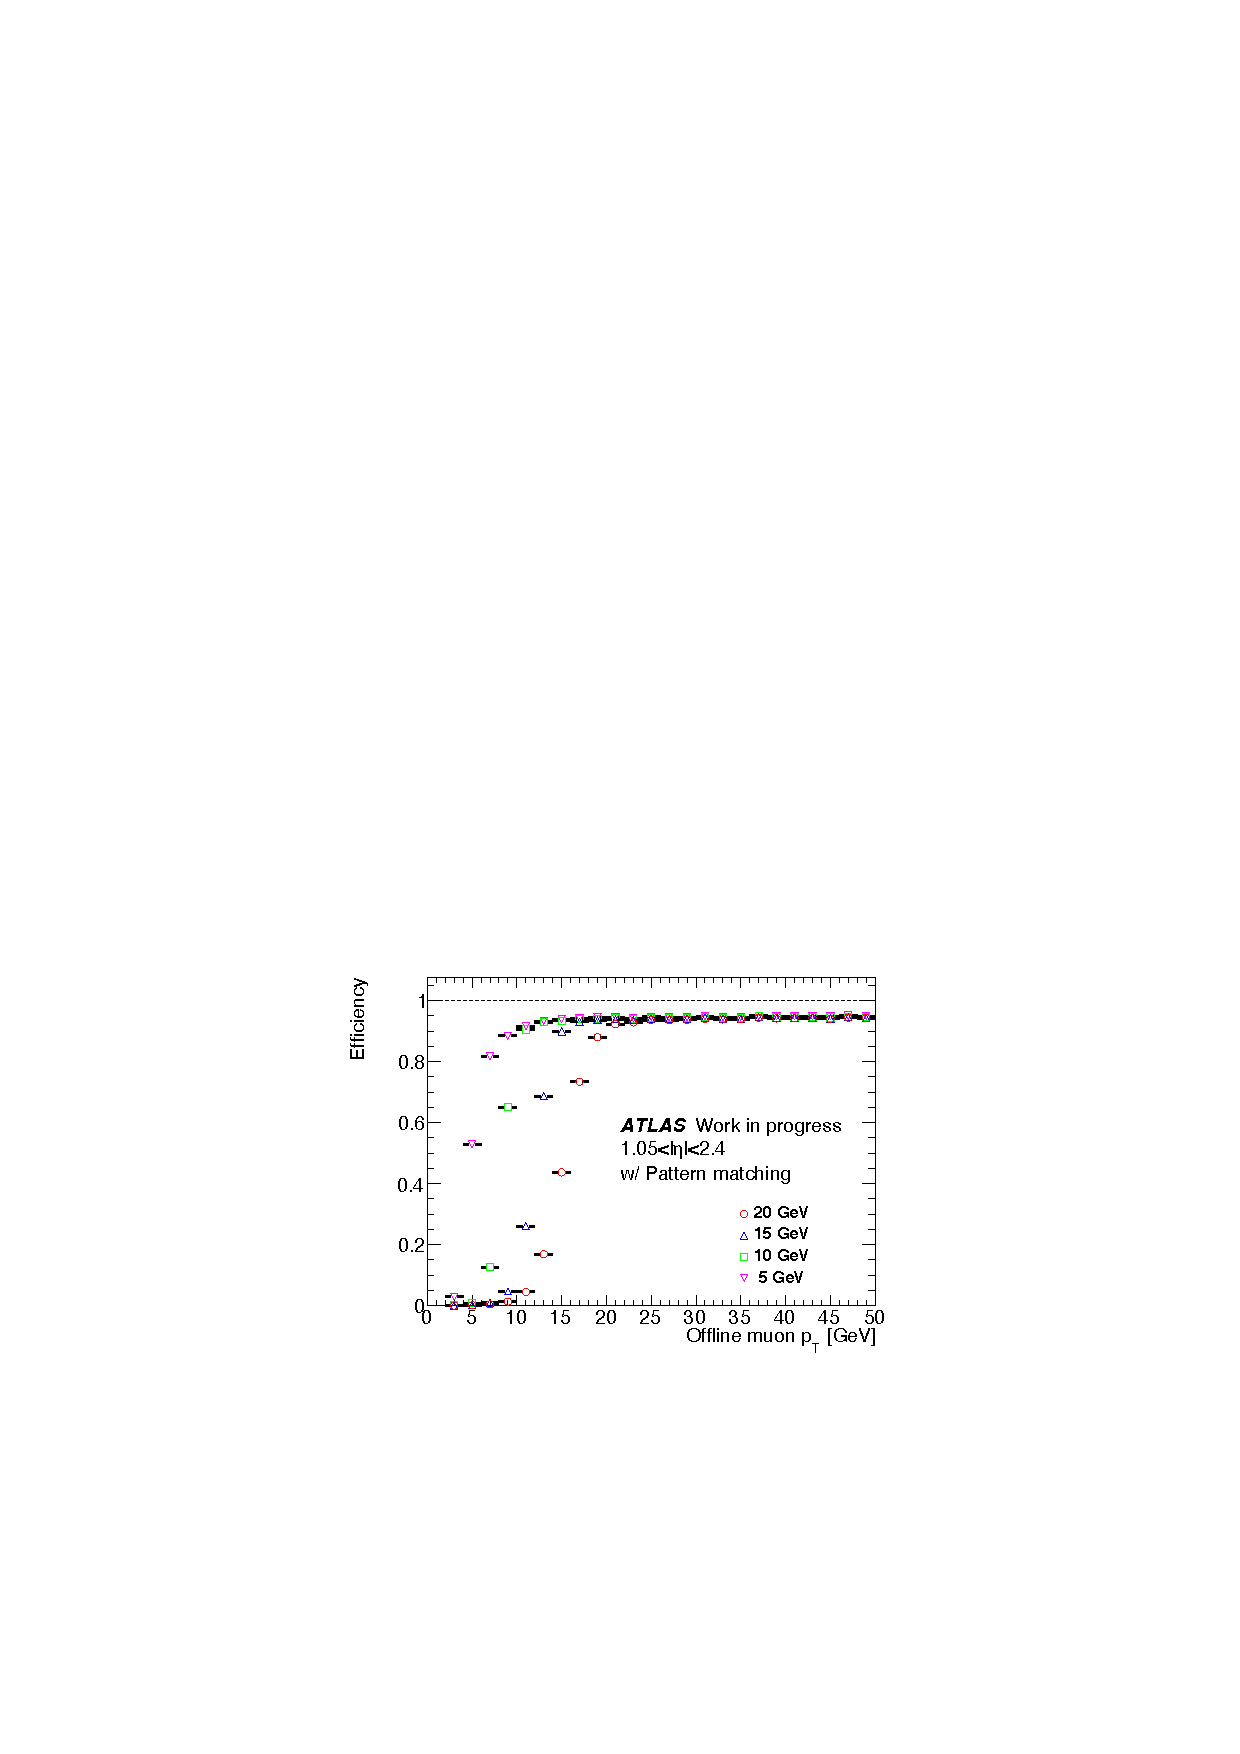
\includegraphics[width=16cm]{fig/Test/Soft_WS.pdf}
    \caption[ソフトウェアシミュレーターで測定された、Wire Strip Coincidenceのトリガー効率]{ソフトウェアシミュレーターで測定された、Wire Strip Coincidenceのトリガー効率\cite{SLPDR}。20 < $p_\mathrm{T}$のプラトー領域でのefficiencyは94 \%程度である。}
    \label{Soft_WS}
\end{figure}


\subsubsection*{Vivado シミュレーターによるWire Segment Reconstructionのトリガー効率測定}
Vivado シミュレーターで測定された、Single Muon  MC に対する Wire Segment Reconstructionのトリガー効率を図\ref{Vivado_Wire_Efficiency}に示す。MCサンプルに含まれるTGC チェンバーのヒットチャンネル情報を、Wire Station Coincidenceのインプットに適したフォーマットに成形した上でVivadoシミュレーションに入力している。Efficiencyは以下のように定義され、Truth Muonの$\eta$、$\phi$ごとにビン分けされている。

\begin{figure}
    \begin{minipage}[b]{.5\linewidth}
    \centering
    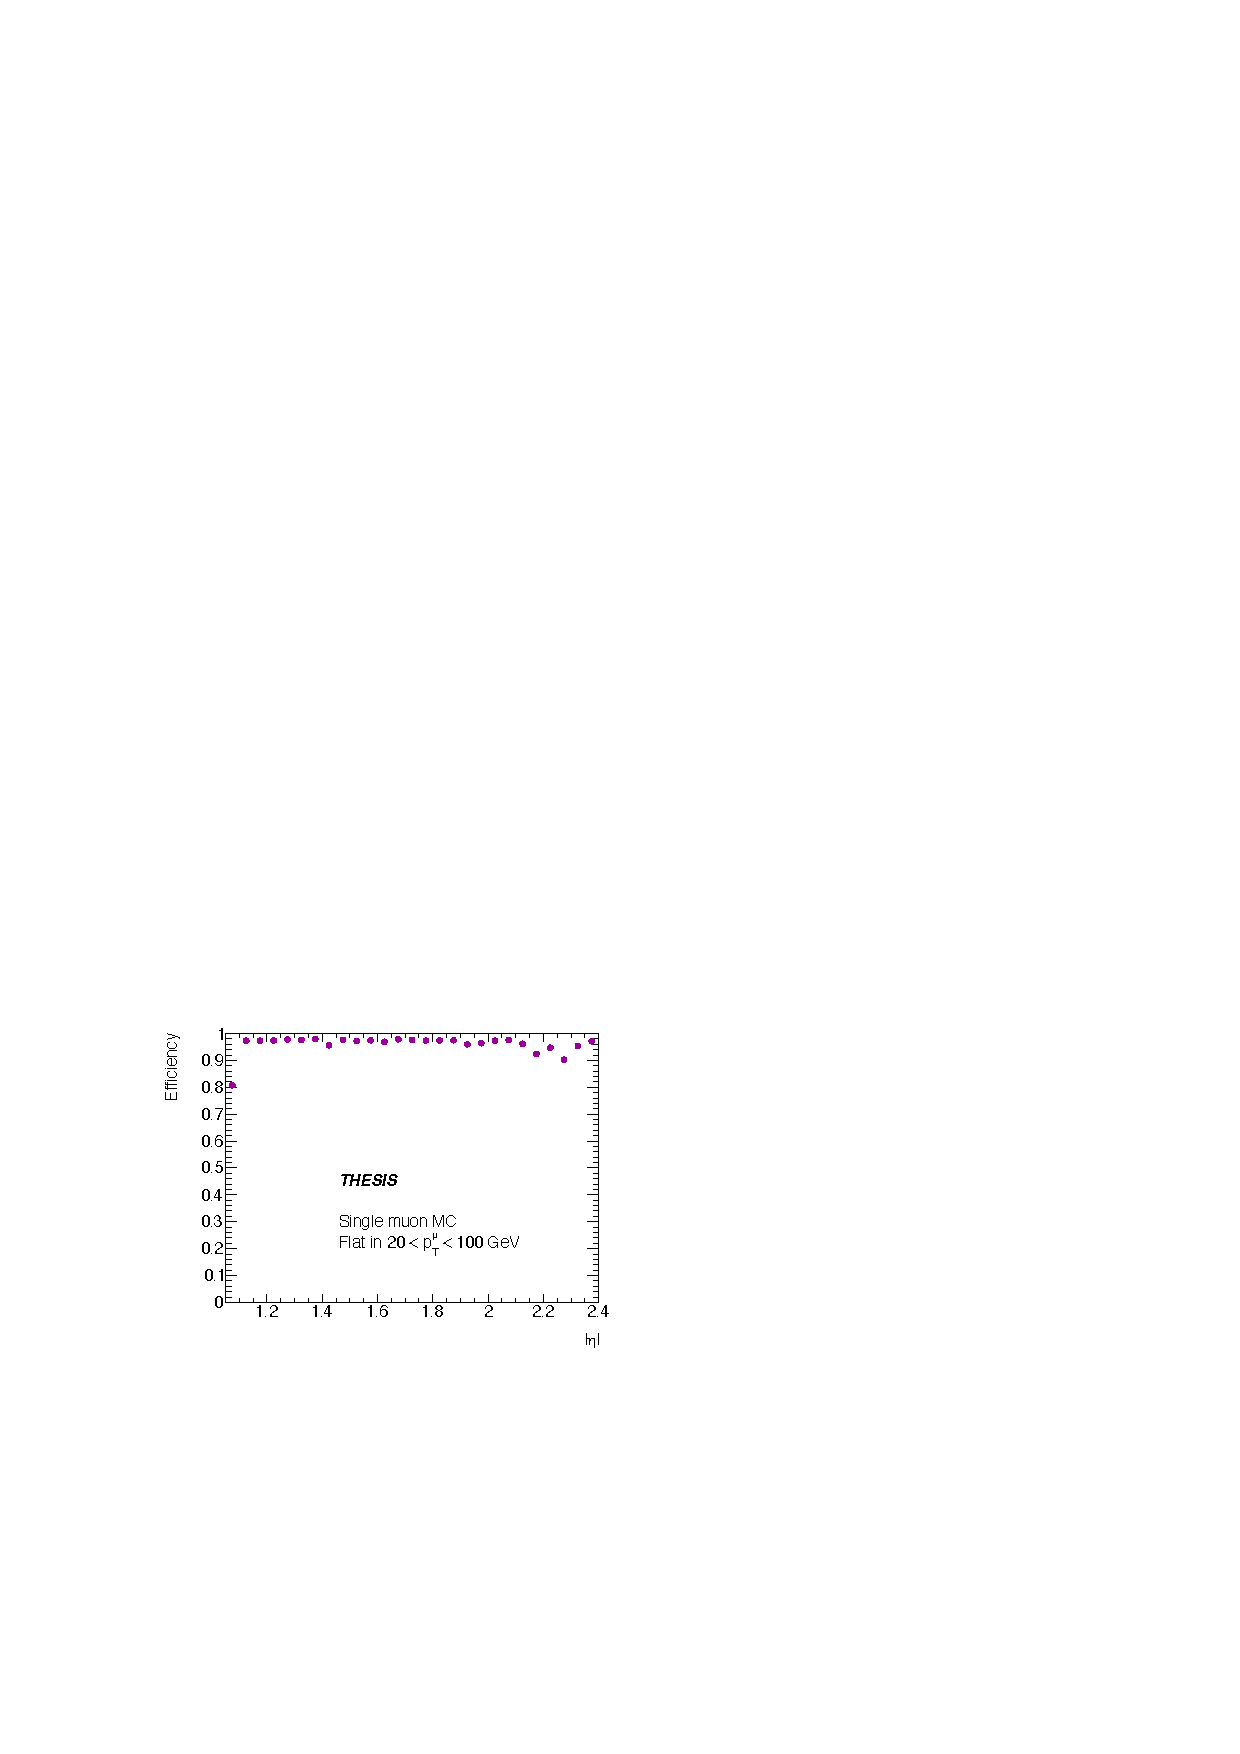
\includegraphics[height=6cm]{fig/Test/Vivado_Wire_eta.pdf}
    \subcaption{Efficiencyの$\eta$依存性}
    \end{minipage}%
    \begin{minipage}[b]{.5\linewidth}
    \centering
    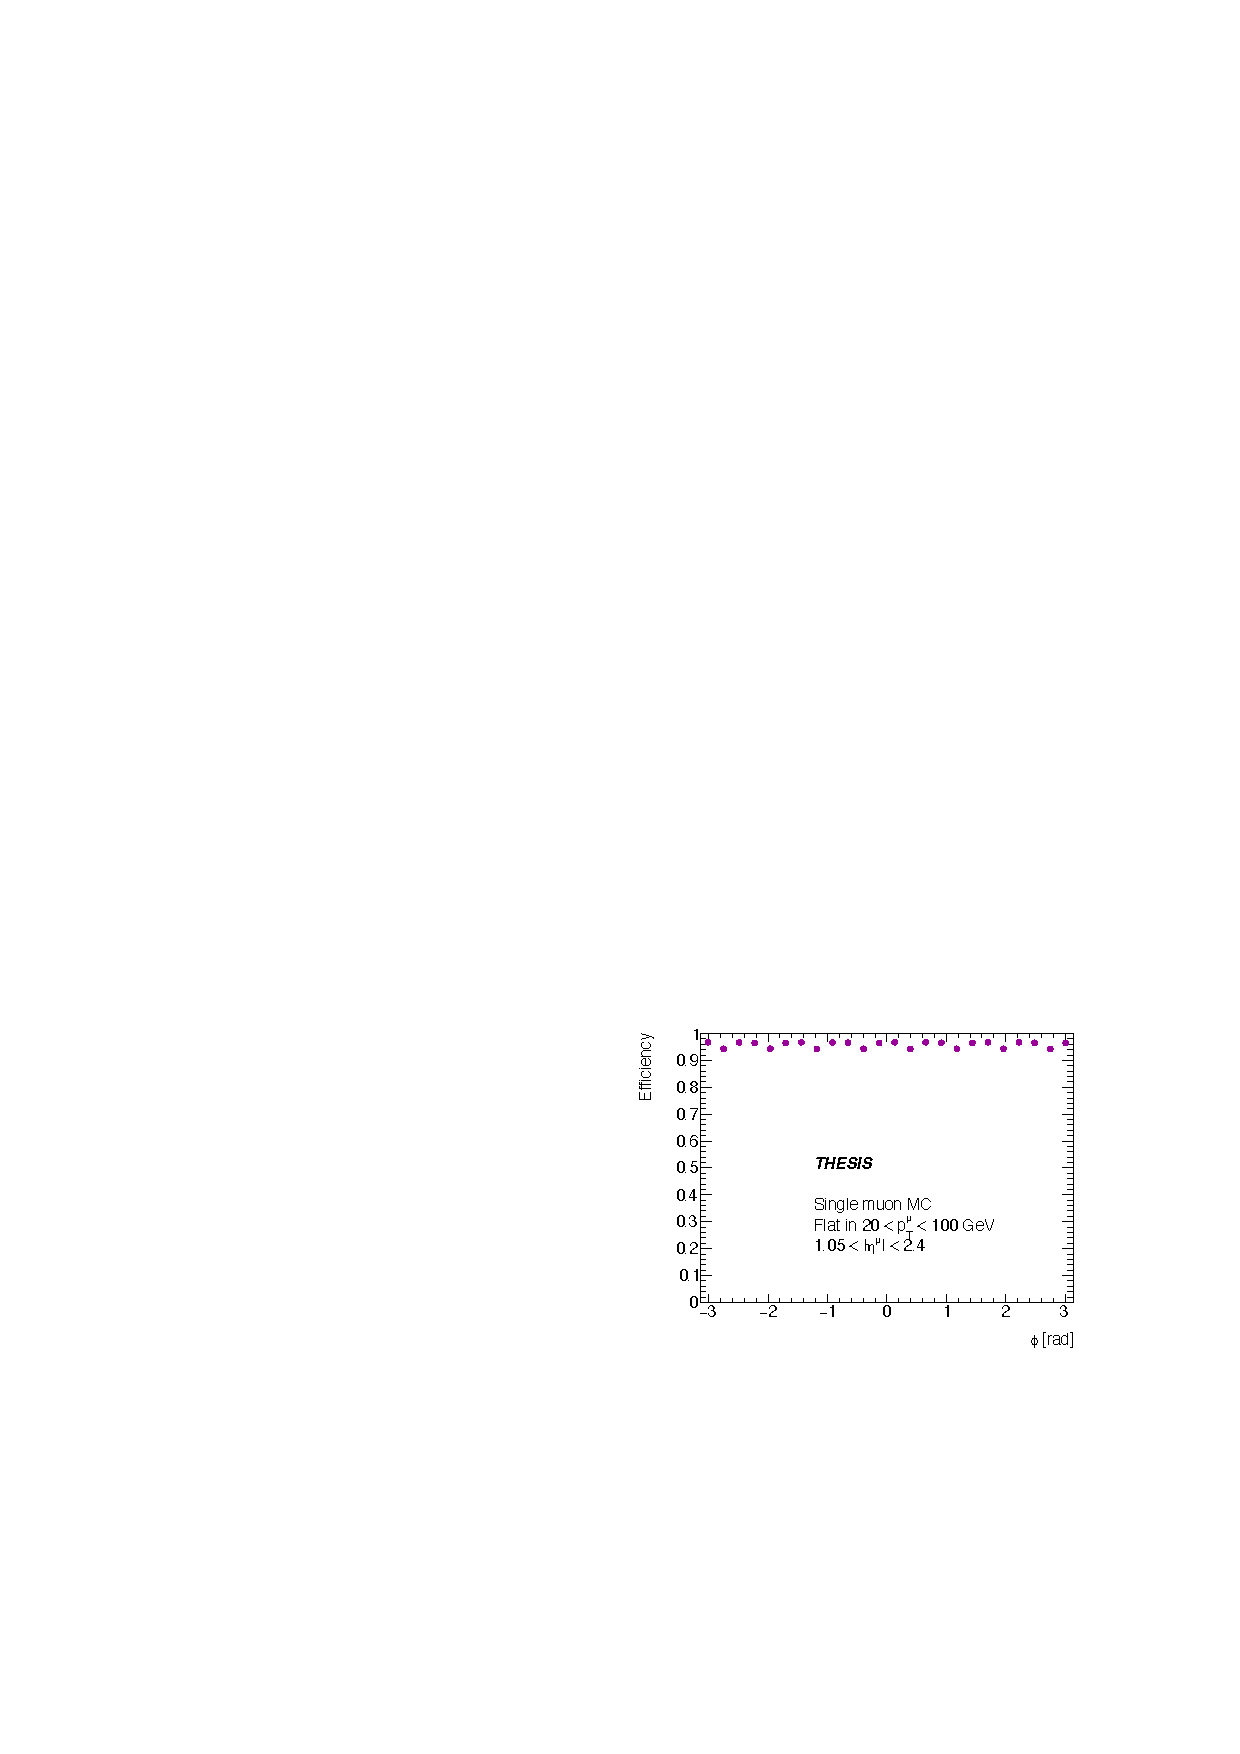
\includegraphics[height=6cm]{fig/Test/Vivado_Wire_phi.pdf}
    \subcaption{Efficiencyの$\phi$依存性}
    \end{minipage}%
    \caption[Wire Segment Reconstructionの検出効率]{Wire Segment Reconstructionの検出効率\cite{mt_nabeyama}。$\eta$、$\phi$全領域でトリガー効率は95 \%程度に達している。}
    \label{Vivado_Wire_Efficiency}
    \end{figure}
    
    \begin{equation}
    \mathrm{Efficiency} = \frac{\mathrm{Wire \,Segment \,Reconstructionで}\,\Delta\theta\,\mathrm{を再構成できたイベント数}}{\mathrm{Truth ミューオン の数}}
\end{equation}

TGCチェンバーの構造やエンドキャップマグネットとの干渉によると考えられる、数\%のInefficiencyが局所的に見られるものの、Efficiencyは$\eta$、$\phi$全領域で95 \%程度に達している。これによりWire Segment Reconstructionの論理回路実装が期待通り達成されていることが検証された。

\subsubsection*{Vivado シミュレーターによるStrip Segment Reconstructionの動作検証}

論理回路実装された Strip Segment Reconstruction と Wire strip Coincidence の動作検証は、ソフトウェアシミュレーター出力との一致を確かめることで行われた。Strip Segment Reconstruction ではソフトウェアシミュレーターによるStrip Station Coincidenceの出力をVivadoシミュレーターの入力とし、出力をソフトウェアシミュレーターと比較している。比較結果を表\ref{tab:Vivado_strip}に示す。エンドキャップ領域 (EC) 、フォワード領域 (FW) それぞれで出力の96 \%程度が一致した。数\%の不一致は、Segment Reconstructionをパスした飛跡候補が複数あった場合にどれを優先的に後段に送るか、という候補選択ロジックの差異によるものであると理解されている。

\begin{table}[]
    \centering
    \caption{Strip Segment Reconstruction出力のソフトウェアシミュレーターとVivadoシミュレーター比較結果}
    \label{tab:Vivado_strip}
    \begin{tabular}{|c|cc|}
    \hline
    \multirow{2}{*}{}        & \multicolumn{2}{c|}{割合}                \\ \cline{2-3} 
                             & \multicolumn{1}{c|}{EC}      & FW      \\ \hline\hline
    飛跡情報が一致したイベント            & \multicolumn{1}{c|}{96.8 \%} & 97.8 \% \\ \hline
    候補の選び方の違いに由来する差異があったイベント & \multicolumn{1}{c|}{3.2 \%}  & 2.2 \%  \\ \hline
    候補の選び方以外に由来する差異があったイベント  & \multicolumn{1}{c|}{1.8 \%}  & 0 \%    \\ \hline
    \end{tabular}
\end{table}



\subsubsection*{Vivado シミュレーターによるWire Strip Reconstructionの動作検証}
Wire Strip Coincidenceの動作検証では、ソフトウェアシミュレーターによるWire Segment ReconstructionとStrip Segment Reconstructionの出力を取り出して、Vivadoシミュレーターの入力としている。比較結果を表\ref{tab:Vivado_WS}に示す。同様のわずかなロジックの違いによる出力の不一致は存在するが、概ねソフトウェアで設計されたロジックと同等のものを論理回路で実装できていることが確認された。

\begin{table}[]
    \centering
    \caption{Wire Strip Coincidence出力のソフトウェアシミュレーターとVivadoシミュレーター比較結果}
    \label{tab:Vivado_WS}
    \begin{tabular}{|c|cc|}
    \hline
    \multirow{2}{*}{}                      & \multicolumn{2}{c|}{割合}                \\ \cline{2-3} 
                                           & \multicolumn{1}{c|}{EC}      & FW      \\ \hline\hline
    飛跡情報が一致したイベント                          & \multicolumn{1}{c|}{98.4 \%} & 99.9 \% \\ \hline
    飛跡情報の異なったイベント                          & \multicolumn{1}{c|}{1.6 \%}  & 0.07 \% \\ \hline
    イベントで最大の\textbackslash{}pt出力がことなったイベント & \multicolumn{1}{c|}{0.09 \%} & 0.02 \% \\ \hline
    \end{tabular}
\end{table}



\clearpage


\section{無限運動量飛跡試験で明らかになった問題点とその修正}
\label{sec:appendix:infinite-momentum-tracks}
無限運動量飛跡の試験で明らかになったトリガー回路の修正点とそのデバッグの過程について述べる。以下にそれぞれのモジュールにおける、修正前の結果と、それに対するデバッグの詳細を示す。


\subsubsection{Strip Segment Reconstructionの結果}
LUT修正前の段階における、無限運動量飛跡に対するStrip Segment Reconstructionの応答を図\ref{Inf_B_Strip}に示す。フォワード領域のStrip スタッガード ID 0番と62番に該当する全ての点で、飛跡再構成に失敗した。この結果は、Bitwiseシミュレーターでも再現された。Bitwiseシミュレーターを用いて詳細な調査を行ったところ、このInefficiencyはLUTに該当するチャンネルの飛跡候補が格納されていないことが原因であると理解された。

この調査の結果をもとにLUTの生成プロセスのデバッグが行われ、この不具合は解消された。
\begin{figure}
    \begin{minipage}[b]{.5\linewidth}
        \centering
        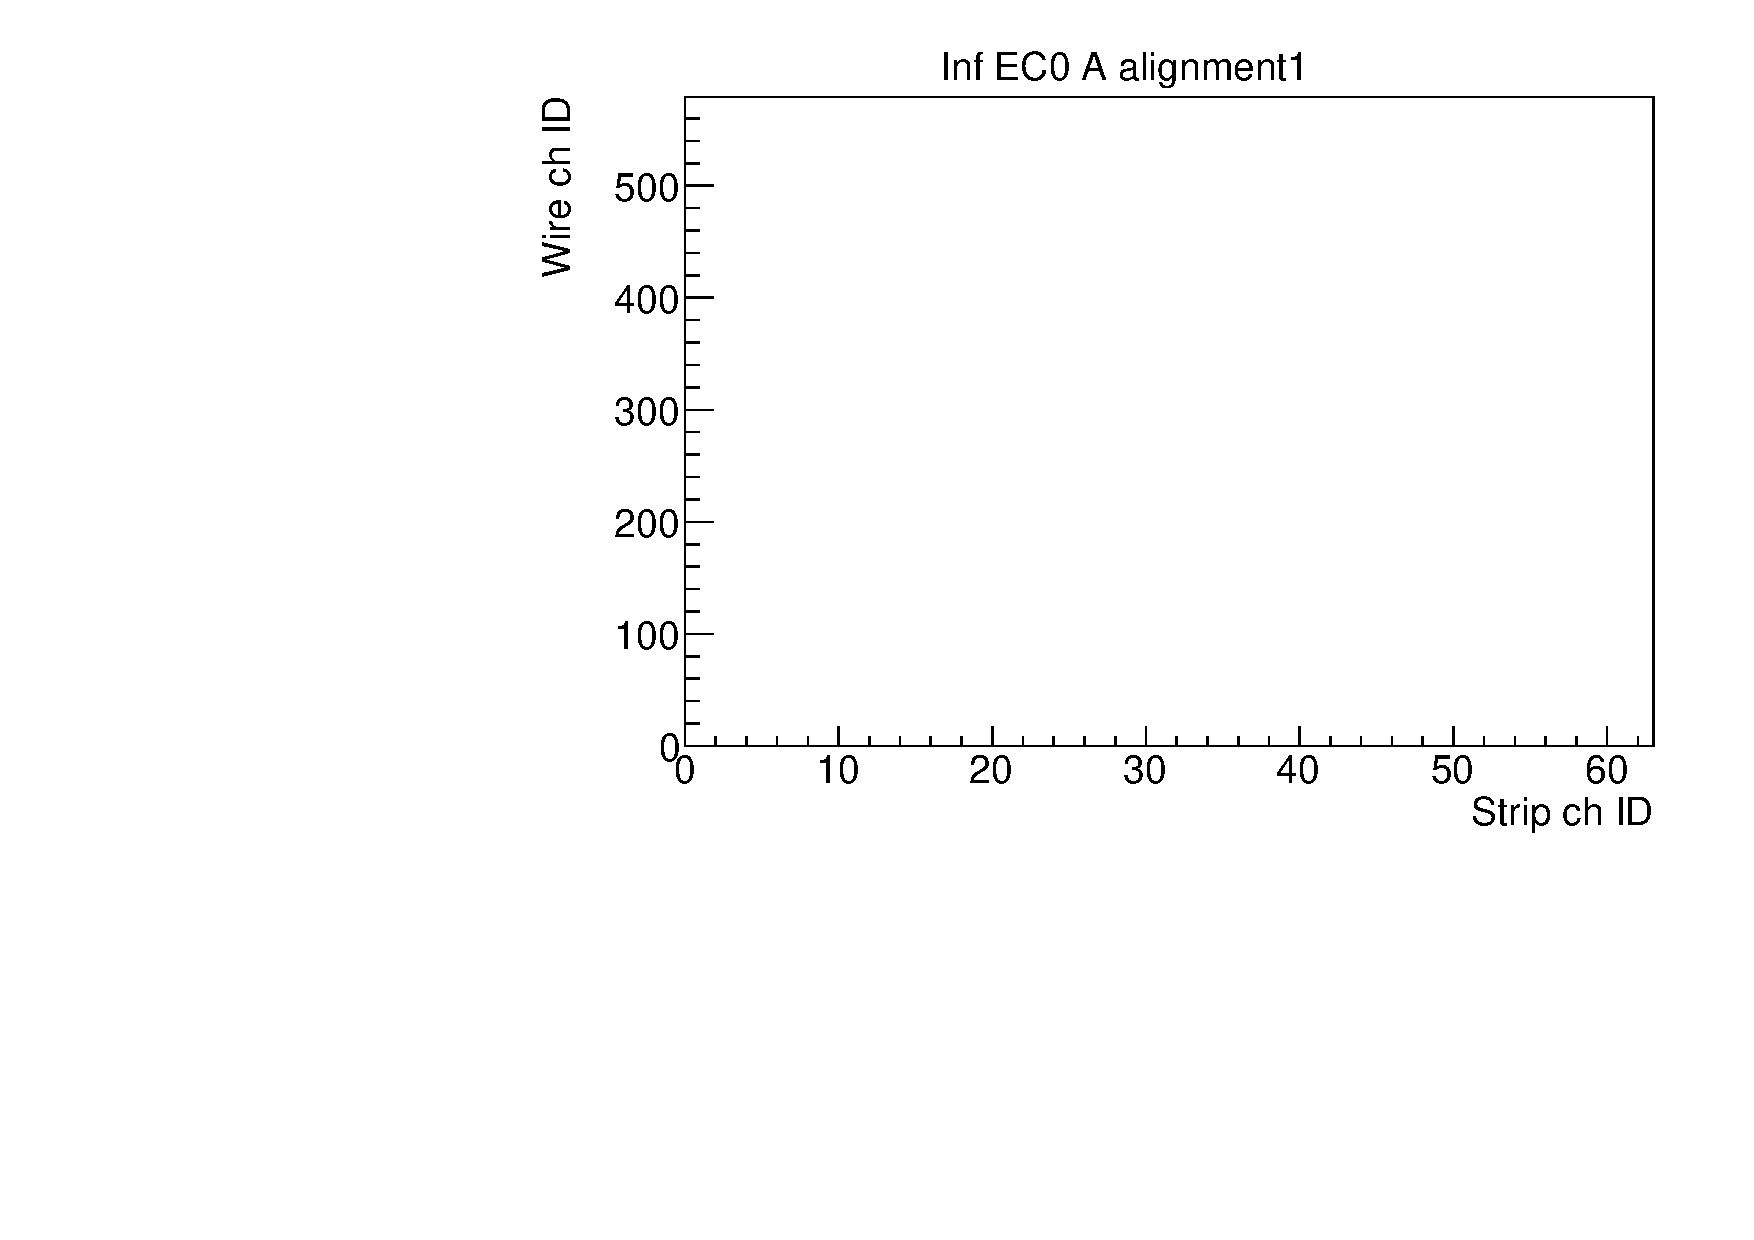
\includegraphics[height=5.6cm]{fig/Test/B_InfEC0_strip.pdf}
        \subcaption{エンドキャップ$\phi\,$0領域の結果}
    \end{minipage}
    \begin{minipage}[b]{.5\linewidth}
        \centering
        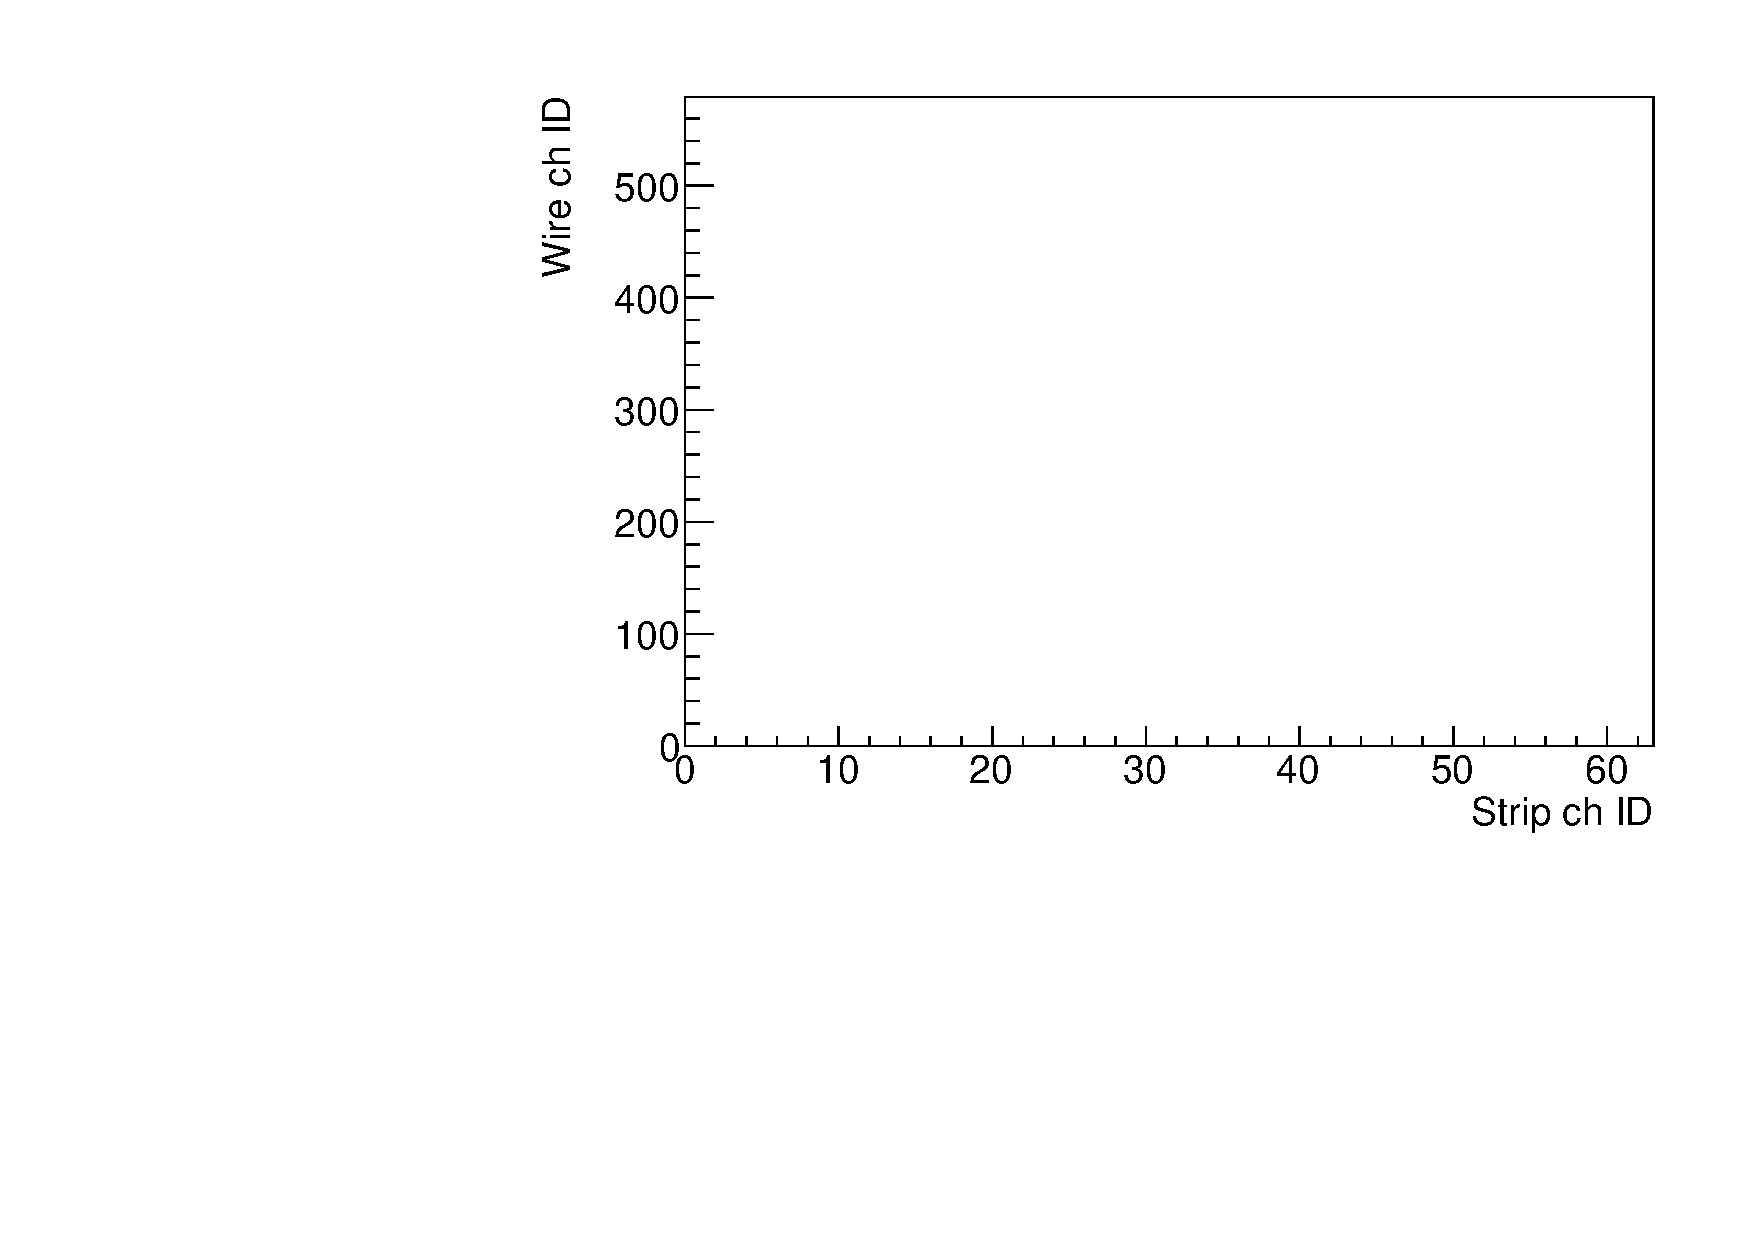
\includegraphics[height=5.6cm]{fig/Test/B_InfEC1_strip.pdf}
        \subcaption{エンドキャップ$\phi\,$1領域の結果}
    \end{minipage}\\
    \begin{minipage}[b]{\linewidth}
        \centering
        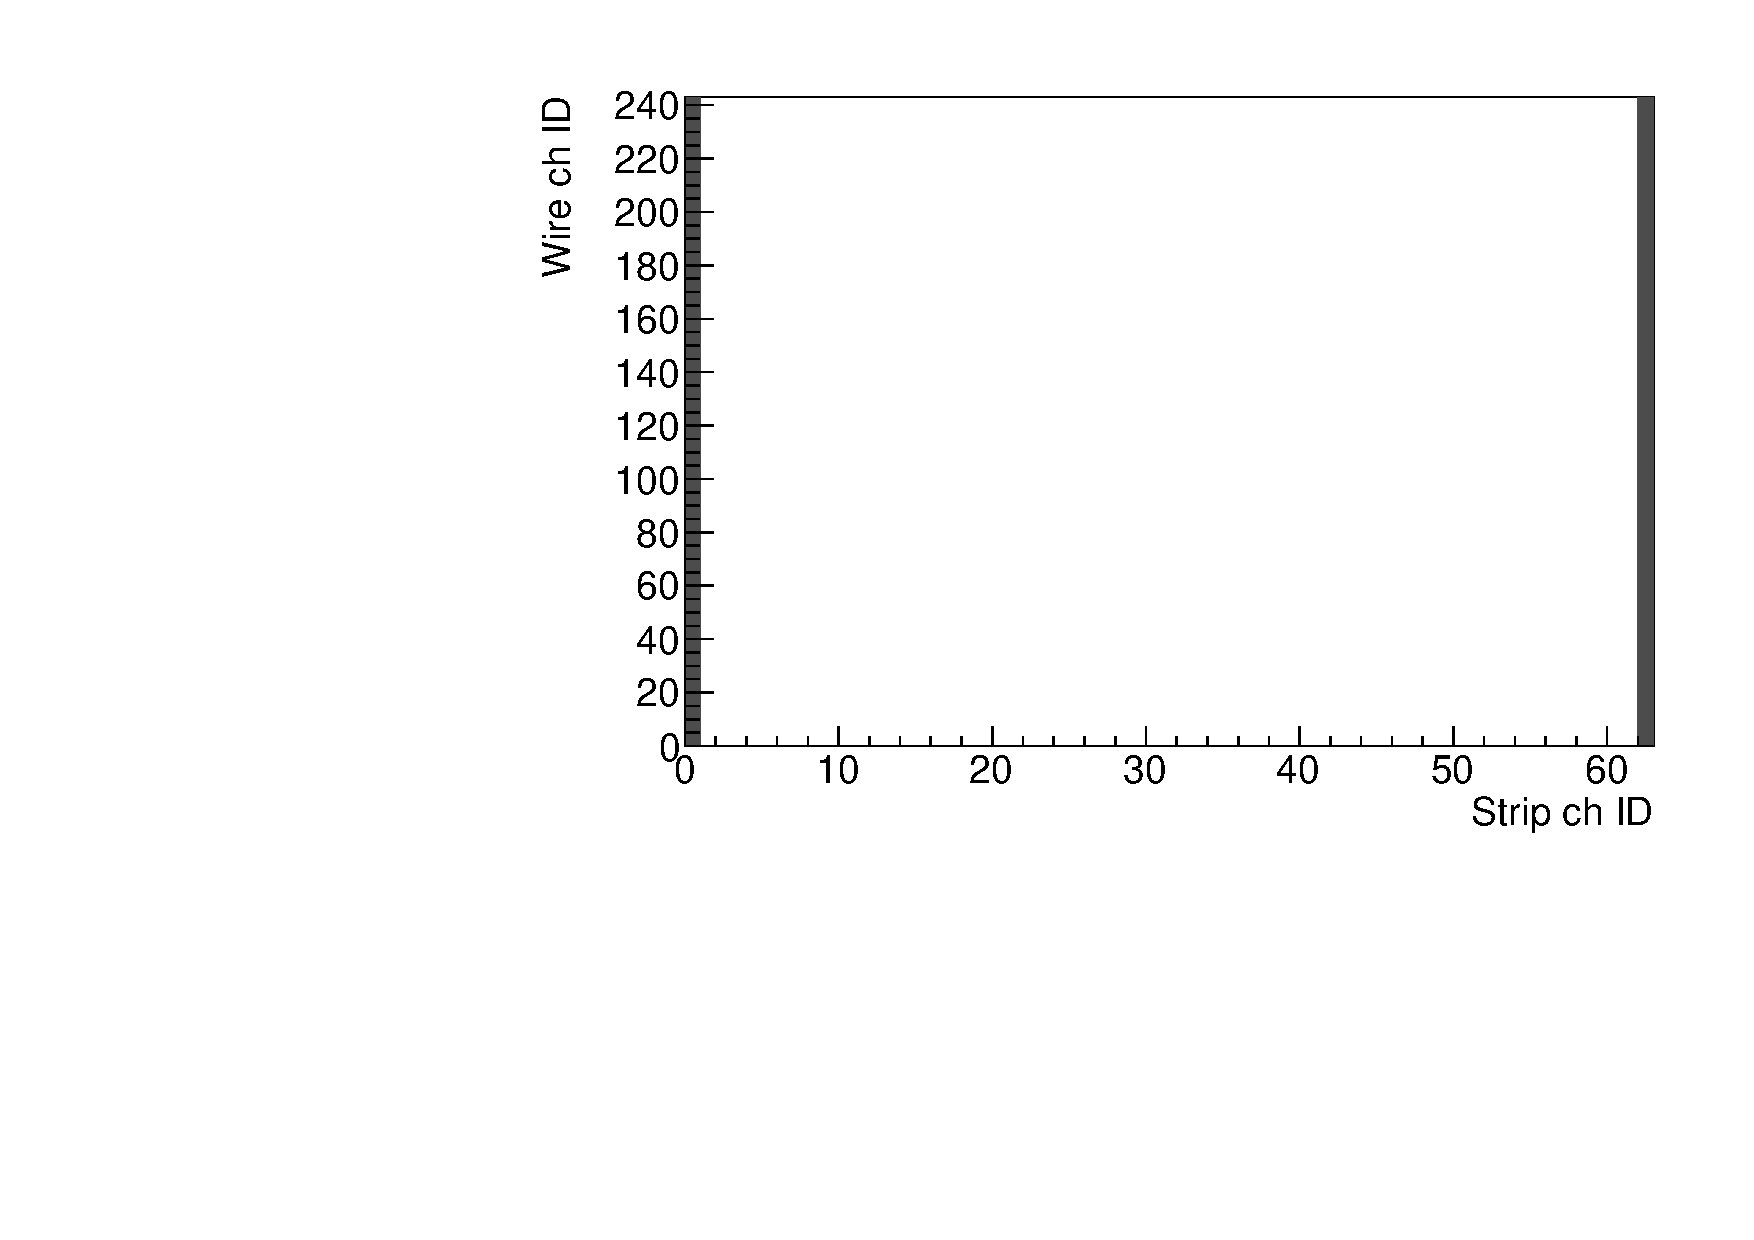
\includegraphics[height=5.6cm]{fig/Test/B_InfFW_strip.pdf}
        \subcaption{フォワード領域の結果}
    \end{minipage}
    \caption[無限運動量飛跡に対する、Strip Segment Reconstructionの応答]{無限運動量飛跡に対する、Strip Segment Reconstructionの応答。横軸にM3におけるStripのスタッガードID、縦軸にM3におけるWireのスタッガードIDをとる。各2次元格子点をピボットとする無限運動量飛跡をシングルボード試験システムに投入し、$0 \leq \Delta\phi$ のSegmentを再構成できた場合にはその格子点を白色、できなかった場合は黒色で塗り潰す。フォワード領域のStrip スタッガード ID 0番と62番に該当する全ての点で、飛跡再構成に失敗している。}
    \label{Inf_B_Strip}
\end{figure}

% \begin{figure} 
%   \centering
%   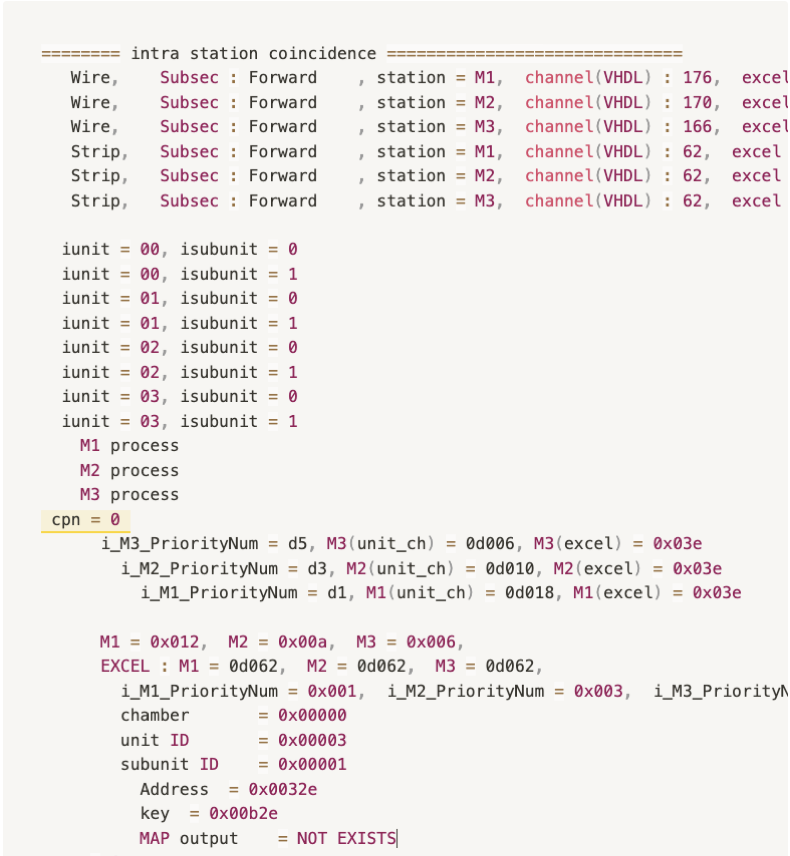
\includegraphics[width=16cm]{fig/Test/Bitwise_example.png}
%   \caption[Strip Segment ReconstructionにおけるBitwiseシミュレーターのログ]{Strip Segment ReconstructionにおけるBitwiseシミュレーターのログ}
%   \label{Bitwise_example}
% \end{figure}

\subsubsection*{Wire Segment Reconstructionの結果}
Wire Segment Reconstructionの結果を図\ref{Inf_B_Wire}に示す。Wire Segment Reconstructionではエンドキャップ領域のWire スタッガードID 200番から350番あたりで大きなInefficiencyが確認された。この不具合は$\eta$ IDの割り振り方の問題によるものであると理解され、ケーブリングデータベースの修正が行われた。もともと、TGC検出器はステーションごとの$\eta$位置分解能が等しくなるように設計されており、設置によるずれが生じた後でも通し番号的に$\eta$ IDを割り振れば同じ$\eta$をカバーするチャンネルを一意に定められると考えられていた。しかし、本試験の結果により、通し番号的に$\eta$ IDを割り振った場合、検出器の中央の領域でステーションごとに$\eta$位置にずれが生じることが明らかになった。

%図\ref{Stag300}に通し番号的に$\eta$ IDを振った場合における、各ステーションの$\eta$ IDの$\eta$位置を示す。左にコインシデンスを取ることができた$\eta$ ID 100 $\sim$ 105までの点を、右にコインシデンスを取ることができなかった$\eta$ ID $\sim$ 305の$\eta$位置を示す。同じ色の点が、同じ$\eta$ IDの代表点を示す。この図から、通し番号的に$\eta$ IDを割り振った場合、$\eta$ ID 300

\begin{figure}
    \begin{minipage}[b]{.5\linewidth}
        \centering
        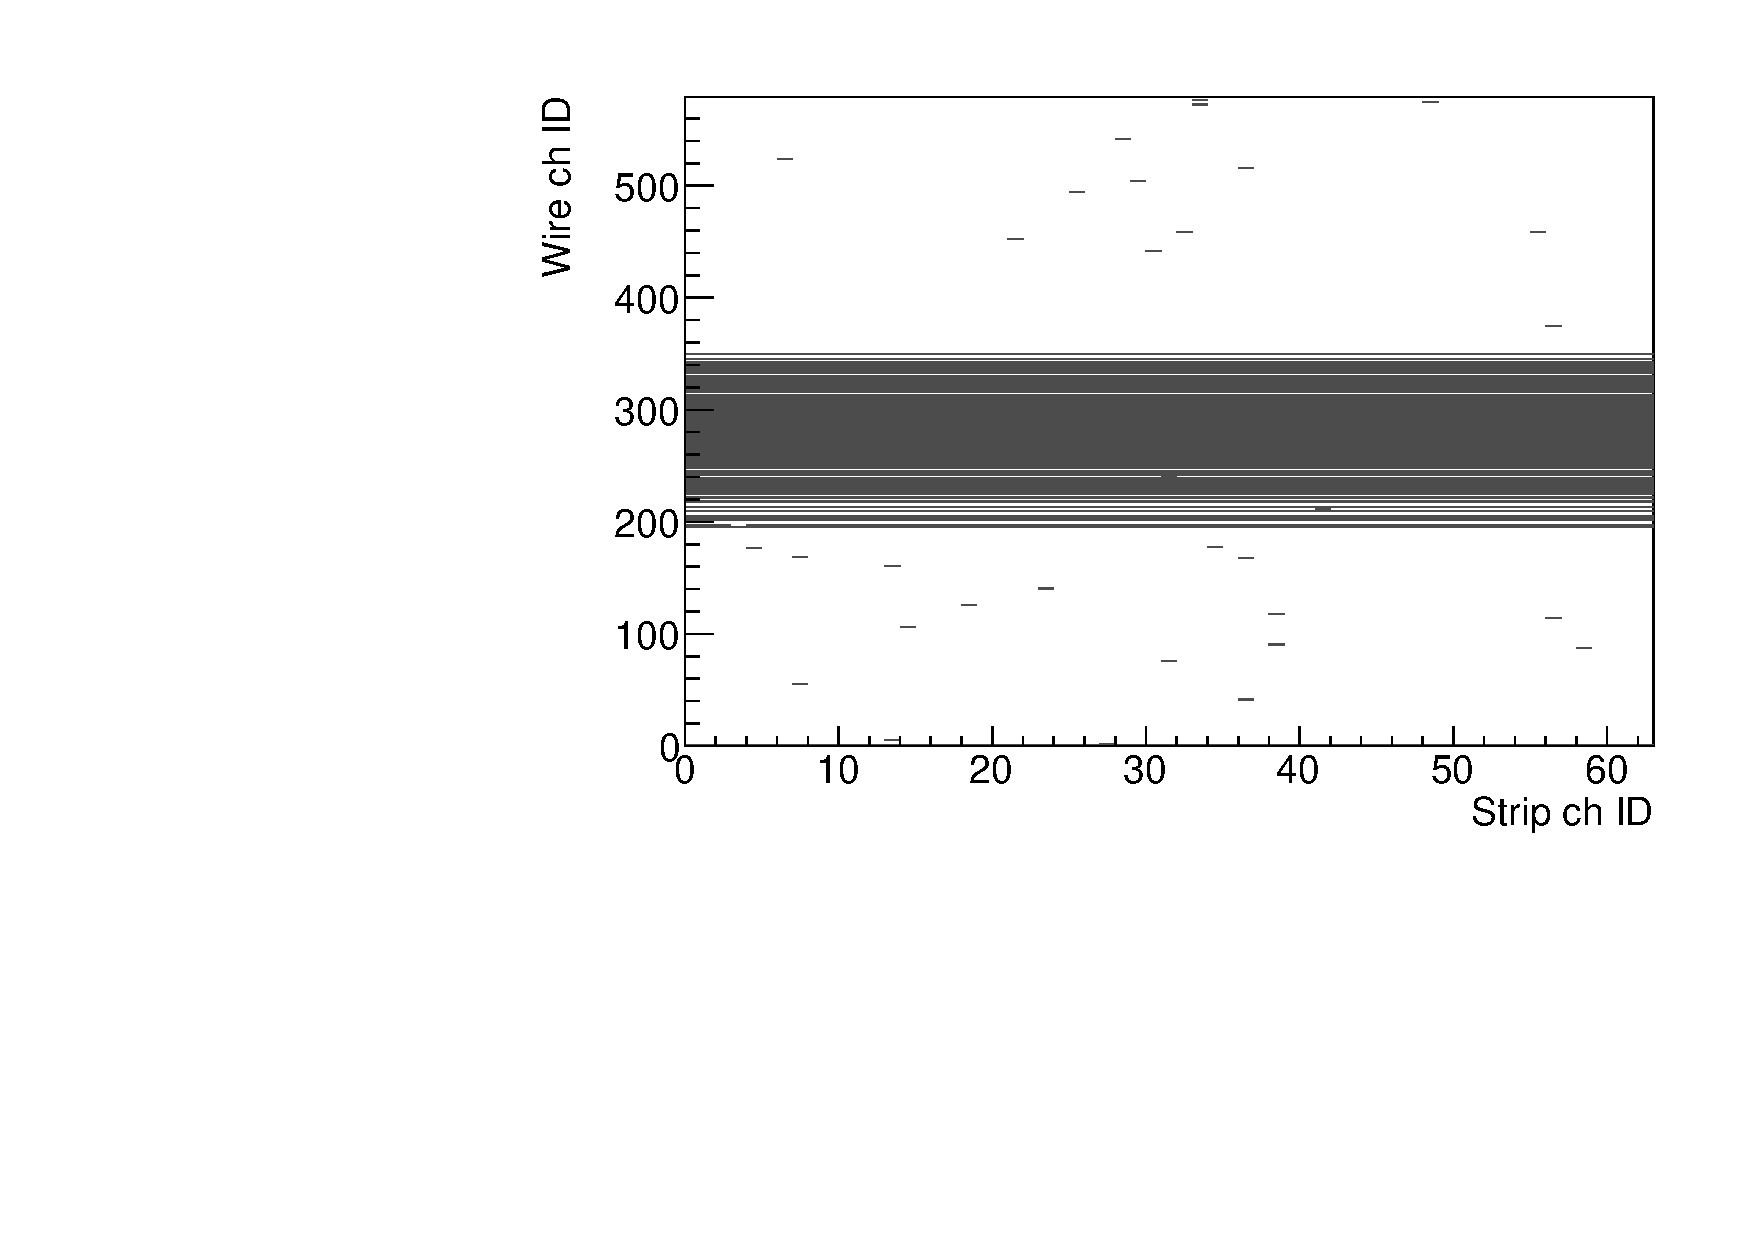
\includegraphics[height=5.6cm]{fig/Test/B_InfEC0_wire.pdf}
        \subcaption{エンドキャップ$\phi\,$0領域の結果}
    \end{minipage}
    \begin{minipage}[b]{.5\linewidth}
        \centering
        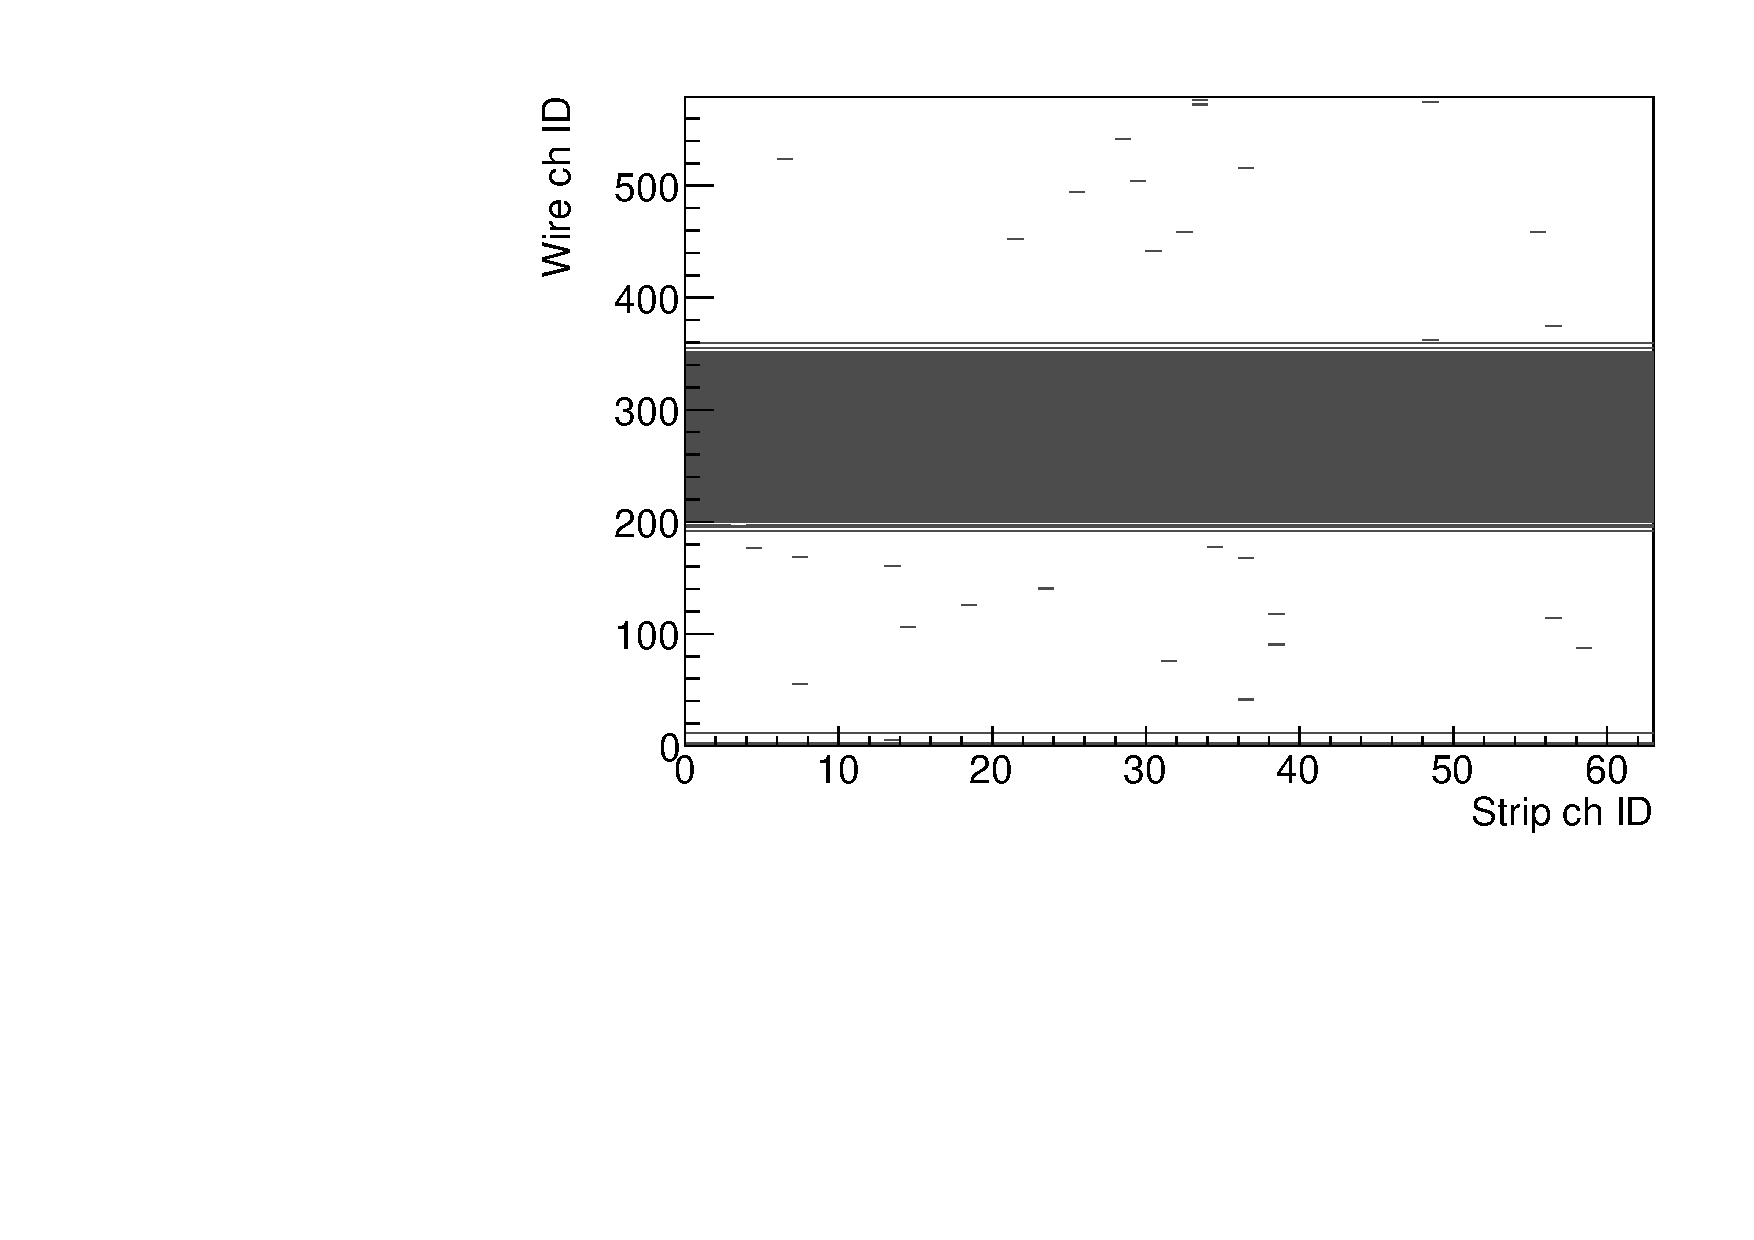
\includegraphics[height=5.6cm]{fig/Test/B_InfEC1_wire.pdf}
        \subcaption{エンドキャップ$\phi\,$1領域の結果}
    \end{minipage}\\
    \begin{minipage}[b]{\linewidth}
        \centering
        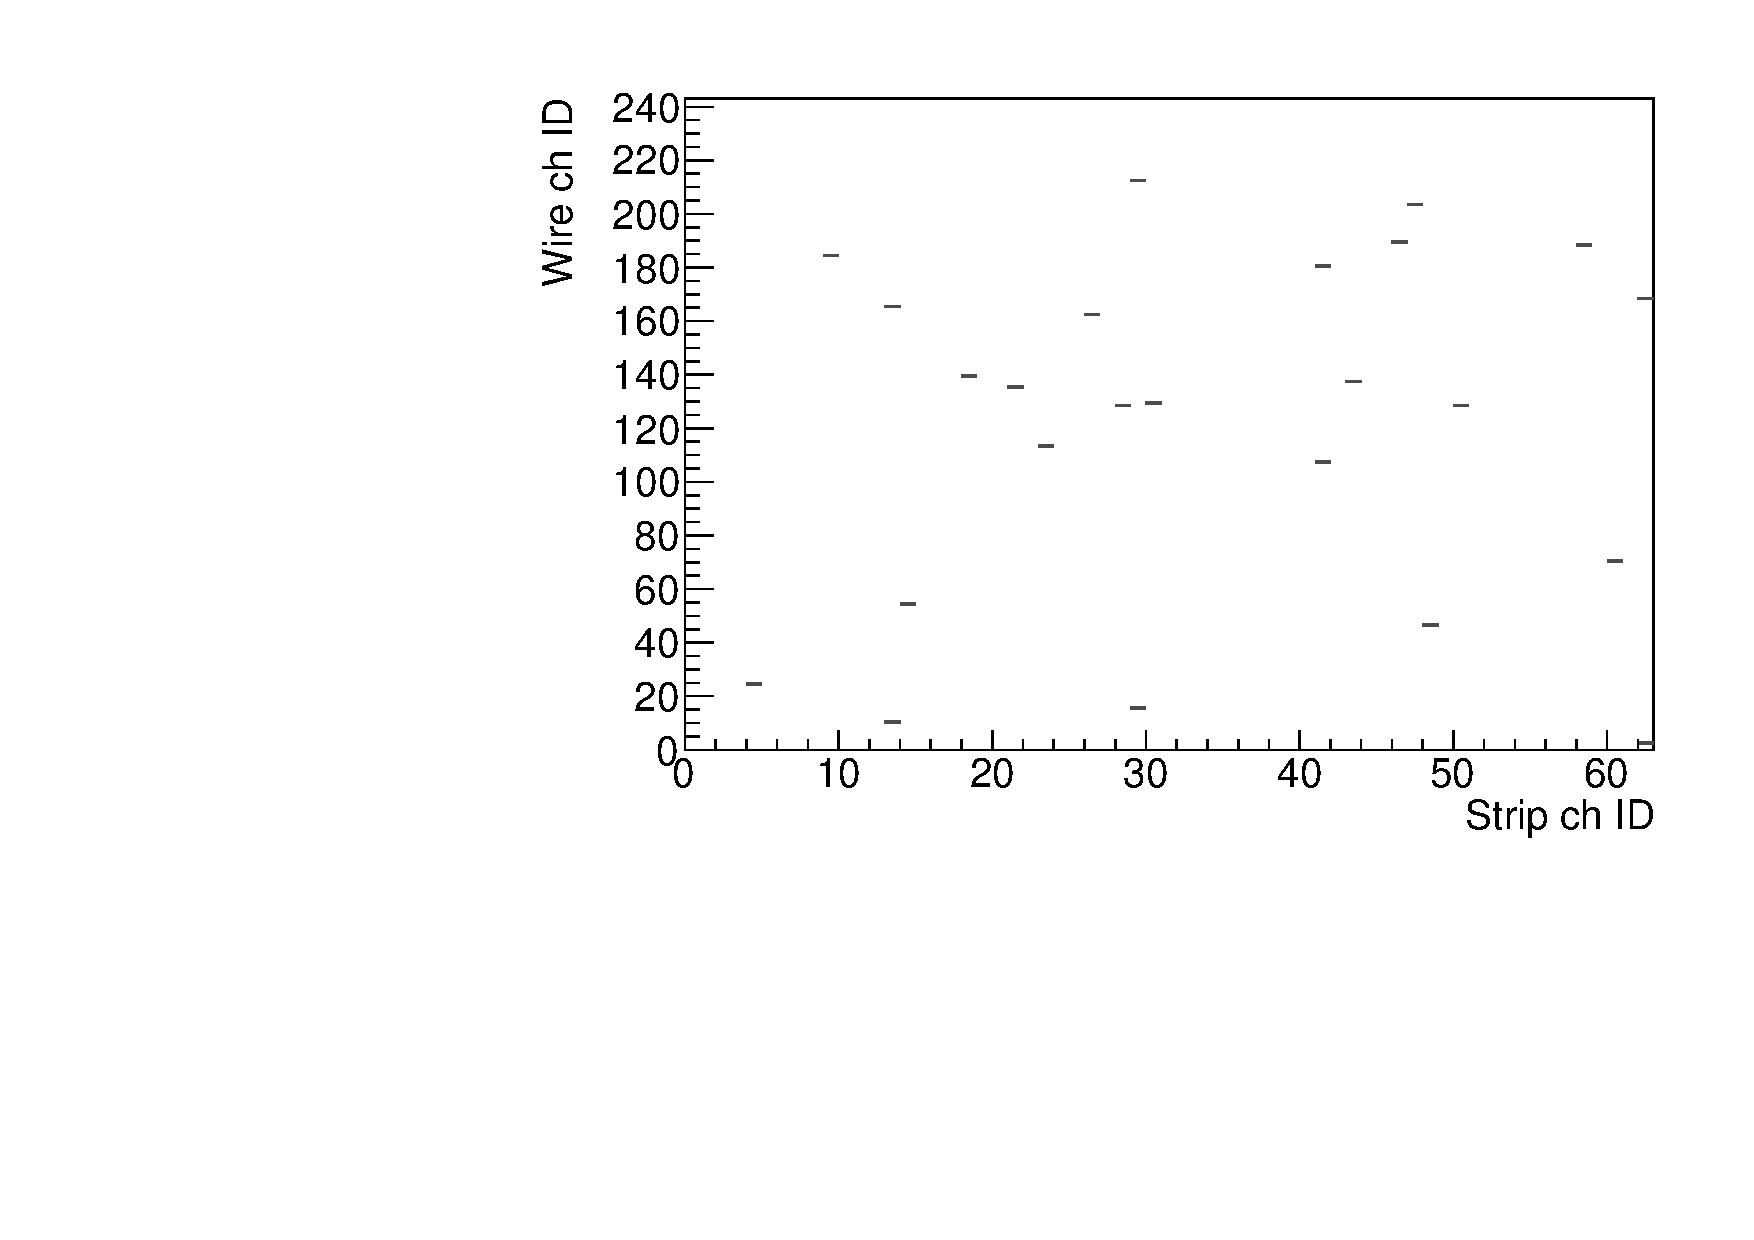
\includegraphics[height=5.6cm]{fig/Test/B_InfFW_wire.pdf}
        \subcaption{フォワード領域の結果}
    \end{minipage}
    \caption[無限運動量飛跡に対する、Wire Segment Reconstructionの応答]{無限運動量飛跡に対する、Wire Segment Reconstructionの応答。横軸にM3におけるStripのスタッガードID、縦軸にM3におけるWireのスタッガードIDをとる。各2次元格子点をピボットとする無限運動量飛跡をシングルボード試験システムに投入し、$0 \leq \Delta\theta$ のSegmentを再構成できた場合にはその格子点を白色、できなかった場合は黒色で塗り潰す。エンドキャップ領域のWire スタッガードID 200番から350番あたりで大きなInefficiencyが確認された。}
    \label{Inf_B_Wire}
\end{figure}

% \begin{figure}
% \begin{minipage}[b]{.5\linewidth}
% \centering
% 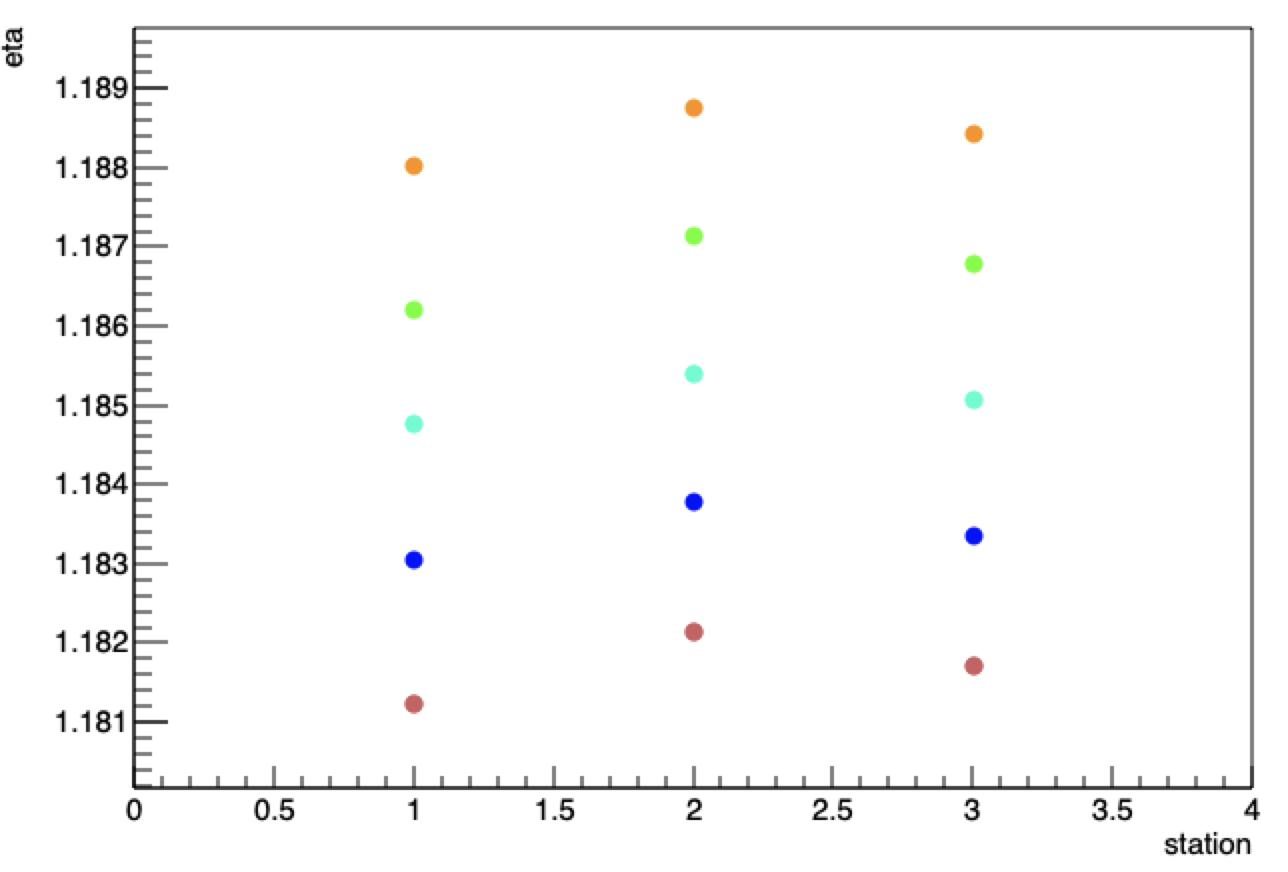
\includegraphics[height=5cm]{fig/Test/Stag100-105.png}
% \subcaption{Wire スタッガードID 100 ~ 105}
% \end{minipage}%
% \begin{minipage}[b]{.5\linewidth}
% \centering
% 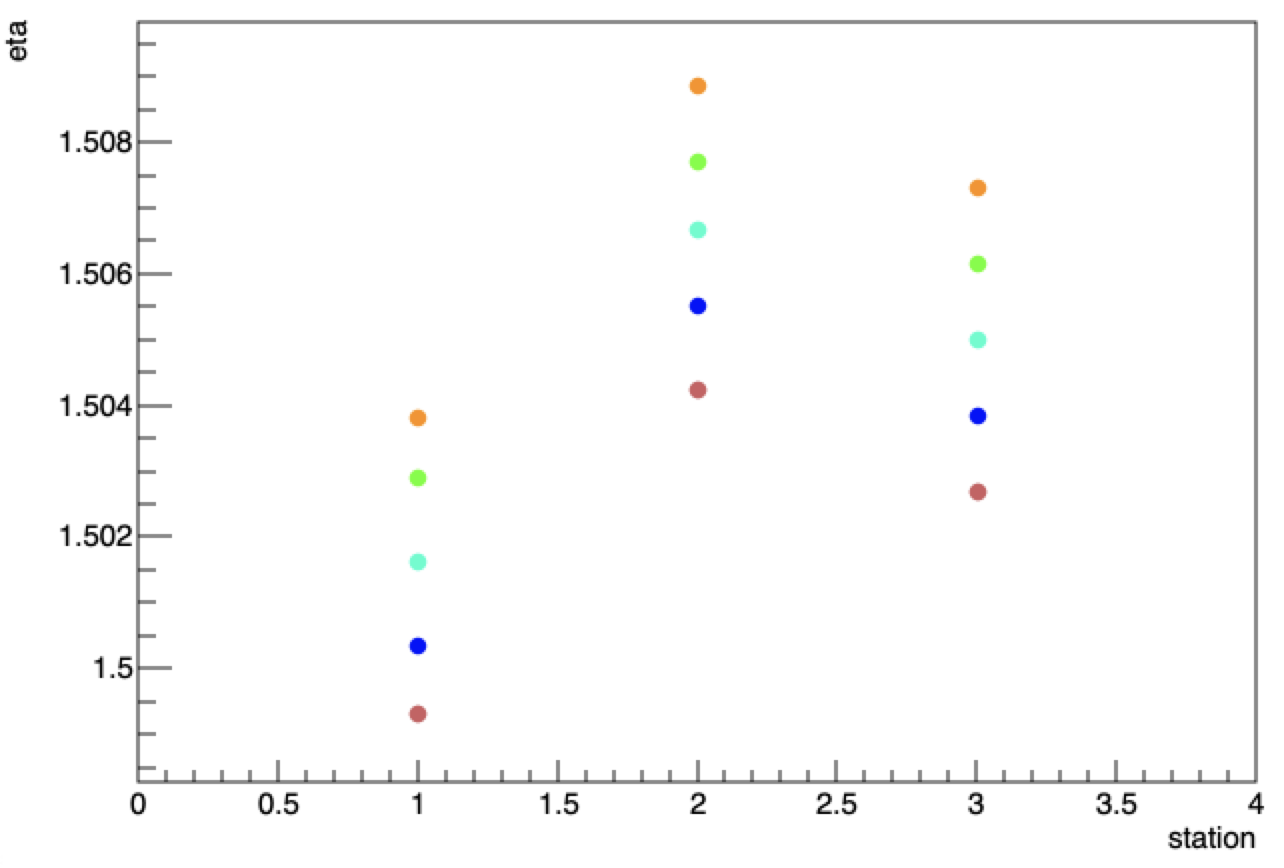
\includegraphics[height=5cm]{fig/Test/Stag300-305.png}
% \subcaption{Wire スタッガードID 300 ~ 305}
% \end{minipage}%
% \caption[Wireでのスタッガードチャンネルのずれ]{通し番号的にスタッガードIDを割り振った場合における、$\eta$位置のずれ。}
% \label{Stag300}
% \end{figure}

\subsubsection*{Wire Strip Coincidenceの結果}
Wire Strip Coincidenceの結果を図\ref{Inf_B_WS}に示す。Wire Strip CoincidenceではStrip Segment Reconstruction、Wire Segment ReconstructionそれぞれのInefficiencyに加えて、Wire スタッガードID 400 番以降の領域で特定の構造を持った不具合が見られる。この不具合については調査と修正が進行中である。

\begin{figure}
    \begin{minipage}[b]{.5\linewidth}
        \centering
        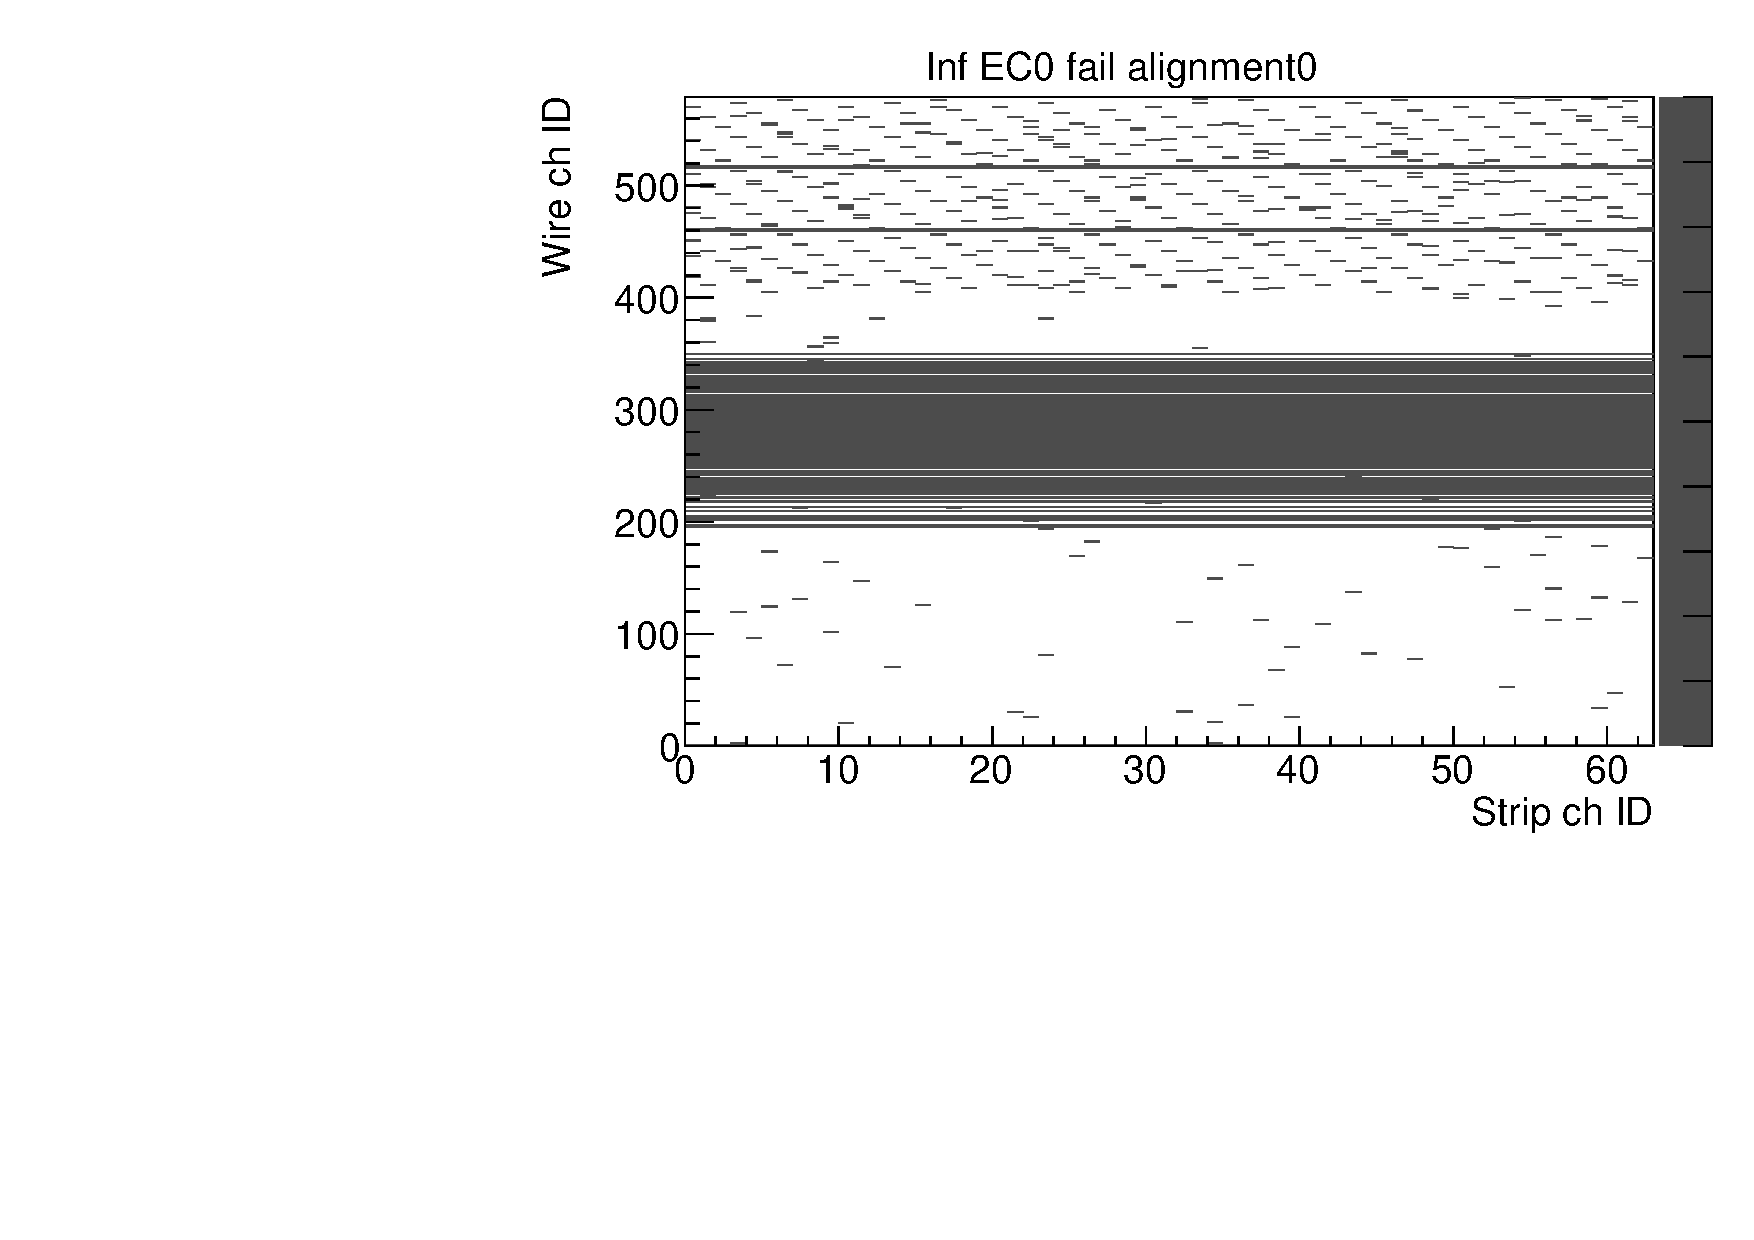
\includegraphics[height=5.6cm]{fig/Test/B_InfEC0_WS.pdf}
        \subcaption{エンドキャップ$\phi\,$0領域の結果}
    \end{minipage}
    \begin{minipage}[b]{.5\linewidth}
        \centering
        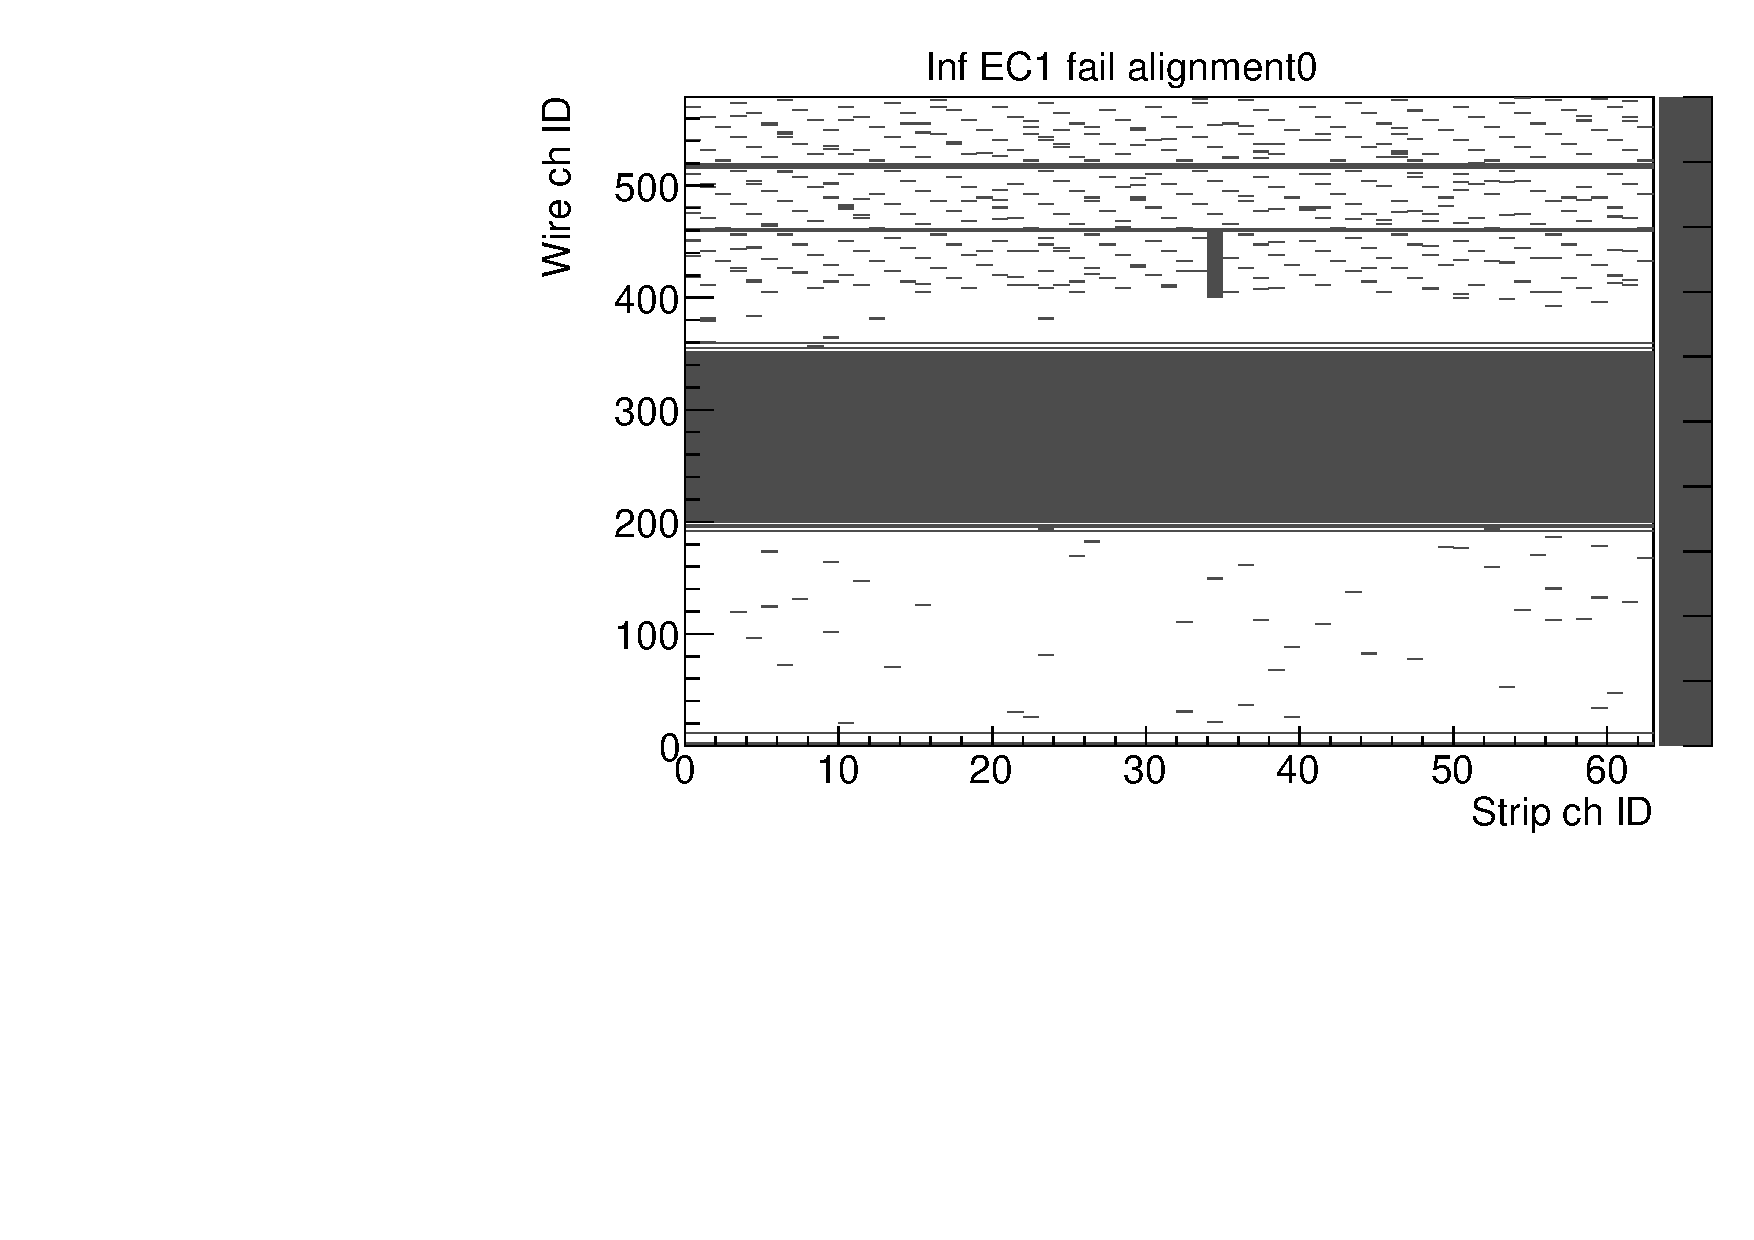
\includegraphics[height=5.6cm]{fig/Test/B_InfEC1_WS.pdf}
        \subcaption{エンドキャップ$\phi\,$1領域の結果}
    \end{minipage}\\
    \begin{minipage}[b]{\linewidth}
        \centering
        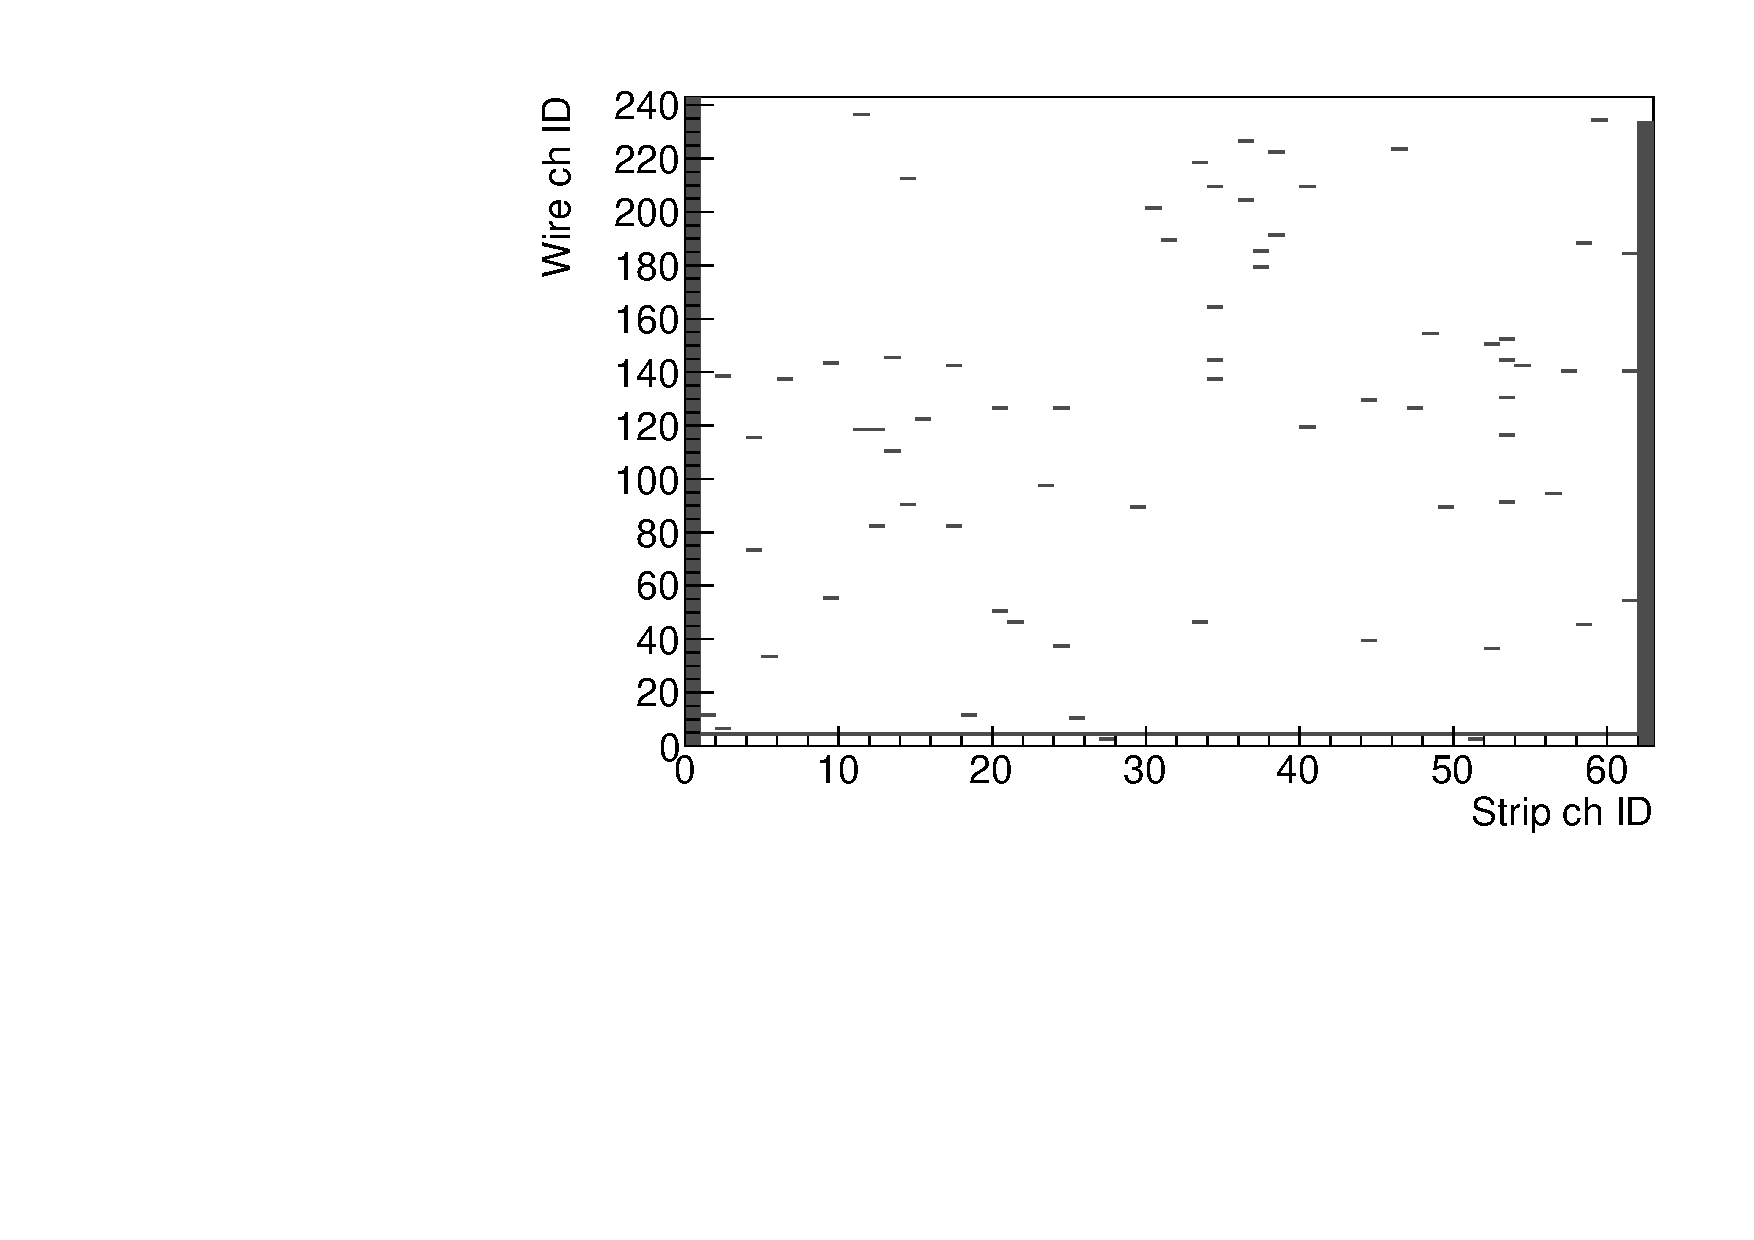
\includegraphics[height=5.6cm]{fig/Test/B_InfFW_WS.pdf}
        \subcaption{フォワード領域の結果}
    \end{minipage}
    \caption[無限運動量飛跡に対する、Wire Strip Coincidenceの応答]{無限運動量飛跡に対する、Wire Strip Coincidenceの応答。横軸にM3におけるStripのスタッガードID、縦軸にM3におけるWireのスタッガードIDをとる。各2次元格子点をピボットとする無限運動量飛跡をシングルボード試験システムに投入し、$0\,\mathrm{GeV} < p_{\mathrm{T}}$ のSegmentを再構成できた場合にはその格子点を白色、できなかった場合は黒色で塗り潰す。Strip Segment Reconstruction、Wire Segment ReconstructionそれぞれのInefficiencyを引き継いでいるほか、Wire スタッガードID 400 番以降の領域で特定の構造を持った不具合が見られる。}
    \label{Inf_B_WS}
\end{figure}




\clearpage
\section{MCデータを用いた試験で明らかになった問題点とその修正}
\label{sec:appendix:MC-test}
\subsubsection{Wire Strip Coincidence}
シングルミューオンMCを用いた試験によって、Wire Strip Coincidenceの\pt 判定に関する不具合を発見した。図\ref{pt_before}にその時の結果を示す。この図では横軸にTruth muonの\pt、縦軸にはWire Strip Coincidenceで判定された\pt 閾値を示す。期待される挙動としては、Truth muon の \pt が5 $\sim$ 10 GeVのイベントはトリガーロジックによって\pt 閾値 5 GeVと判定される。しかし、実際はTruth $p_\mathrm{T}$ が5 GeVや10 GeVのイベントの多くが、$p_\mathrm{T}$閾値 20 GeVと判定されていることがわかる。

\begin{figure} 
\centering
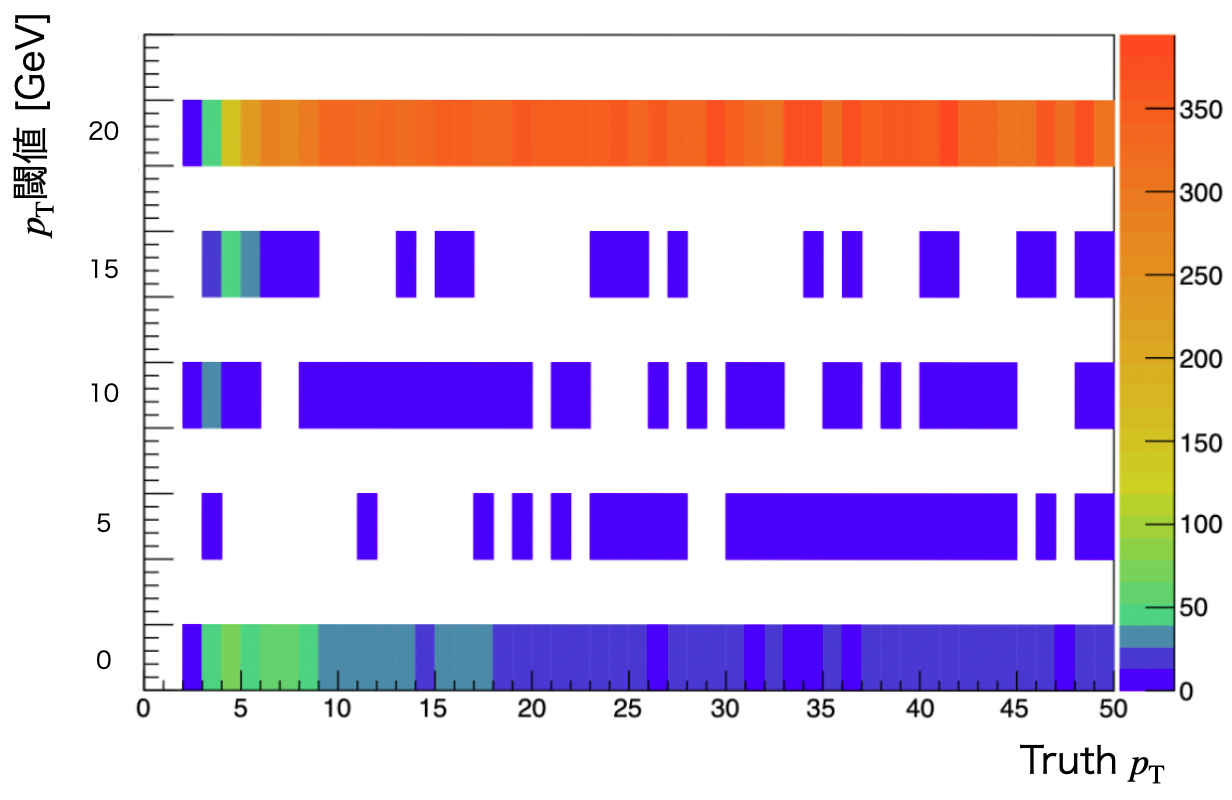
\includegraphics[width=16cm]{fig/Test/pt_before.png}
\caption[]{Wire LUT修正前のTruth $p_\mathrm{T}$とWire Strip Coincidenceで判定された$p_\mathrm{T}$の関係。Truth $p_\mathrm{T}$ が5 GeVや10 GeVのイベントの多くが、$p_\mathrm{T}$閾値 20 GeVと判定されており、正しく\pt 判定がなされていないことがわかる。}
\label{pt_before}
\end{figure}

この問題のデバッグを行ったところ、Wire Segment Reconstructionの出力として定義される$\Delta\theta$の単位系とWire Strip Coincidenceの入力として定義される$\Delta\theta$の単位系が異なっていることが明らかになった。Wire Segment reconstructionでは$\Delta\theta$は4 mrad区切りの整数値として定義され、Wire Strip Coincidenceでは1.25 mrad区切りの整数値として定義されていた。
そのため、例えばTruthの$\Delta\theta$が10 mradの場合、WireSegmnet Reconstructionの出力は"2"である。一方、Wire Strip Coincidenceではそれを$1.25 \times 2 = 25\,\mathrm{mrad}$と解釈する。これにより、Truthの\pt が小さく、$\Delta\theta$が大きいイベントに対しても高い\pt 閾値判定を行ってしまっていた。
この不具合の修正のため、Wire Strip Coincidenceの高い分解能に合わせる形でWire LUTを作り直した。その結果を図\ref{pt_after}に示す。Wire Strip CoincidenceではTruth $p_\mathrm{T}$と矛盾のない$p_\mathrm{T}$ 閾値が判定なされるようになった。
 
\begin{figure} 
\centering
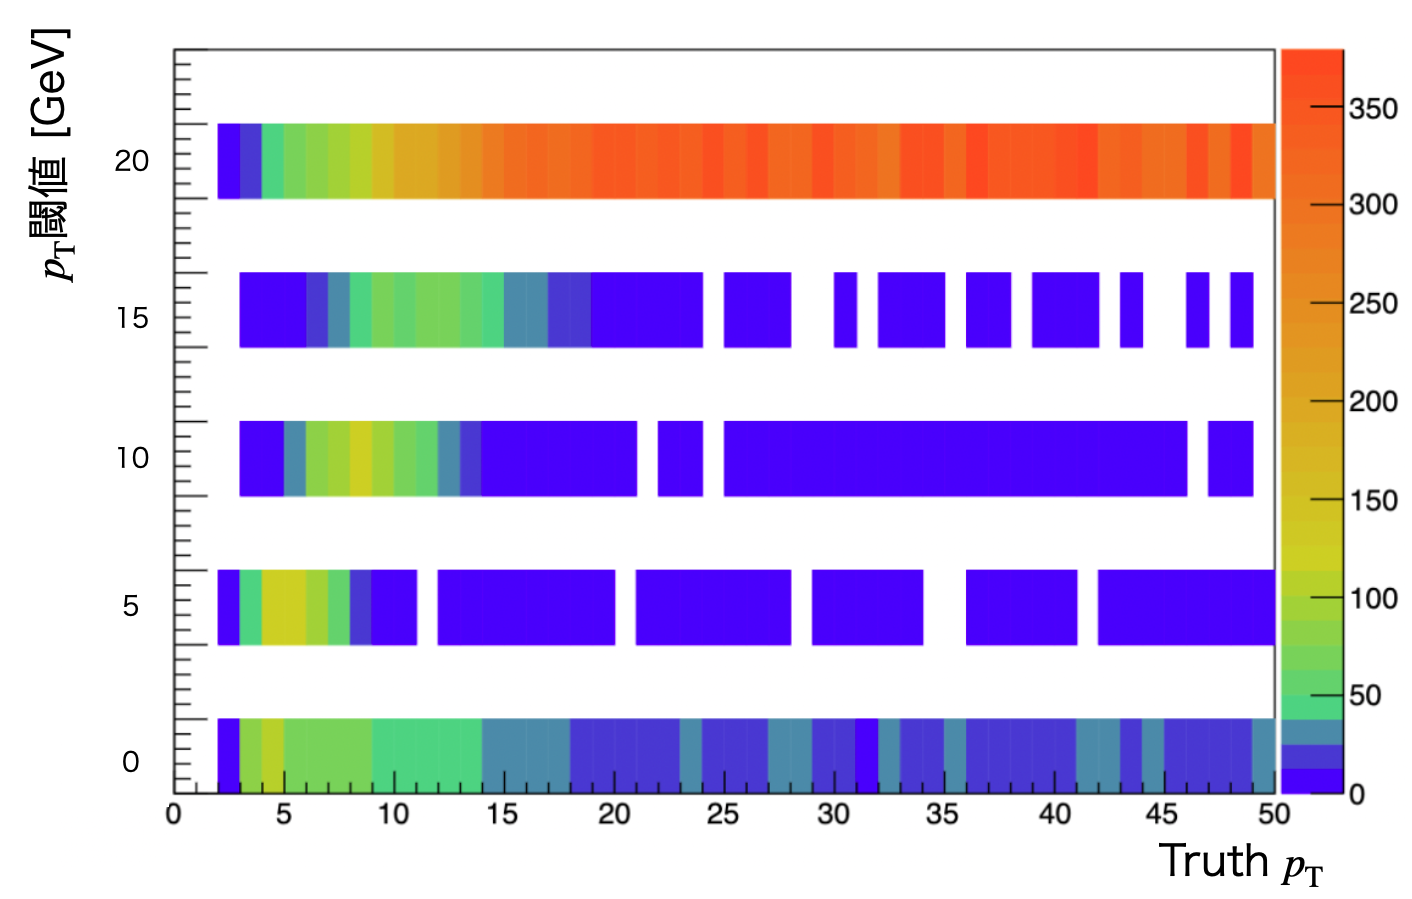
\includegraphics[width=16cm]{fig/Test/pt_after.png}
\caption[]{Wire LUT修正後のTruth $p_\mathrm{T}$とWire Strip Coincidenceで判定された$p_\mathrm{T}$の関係。Wire Strip CoincidenceにおいてTruth $p_\mathrm{T}$と矛盾のない$p_\mathrm{T}$ 閾値が出力されている。}
\label{pt_after}
\end{figure}






\clearpage
\section{プラトー領域におけるInefficiencyの調査}
\label{sec:appendix:plateau}
図\ref{SM_A_WS_turnon}で示した、シングルミューオンモンテカルロデータを用いたトリガー効率測定によると、Truth \pt が 20 GeVより大きいプラトー領域においてもトリガー効率は94 \%程度であり、Truthの\pt によらず6 \%程度のInefficiencyが見られる。本節ではこのInefficiencyの原因について考察する。

Inefficiencyの原因として主に以下の2つが考えられる。1つ目はTGC検出器のミューオン検出効率が100 \%ではないことによるInefficiencyである。高輝度LHC-ATLAS実験でのトリガーロジックはワイヤーでは7層中5層かつ各ステーションに少なくても1つヒットがあること、ストリップでは6層中4層かつ各ステーションに少なくても1つヒットがあること、が要求される。そのため、例えばミューオンがM2の2層ともヒットを残さず、素通りしたとすると飛跡を再構成することはできない。2017年の運転におけるTGC各層のヒット検出効率分布を図\ref{tgchit_efficiency}に示す。1枚のガスレイヤーにおけるヒット検出効率の平均はワイヤーで92.7 \%、ストリップで92.1 \%程度であり、100 \%ではない。そのため、ある一定以上の確率でこのような避けられないInefficiencyが生じる。

\begin{figure}
\begin{minipage}[b]{.5\linewidth}
\centering
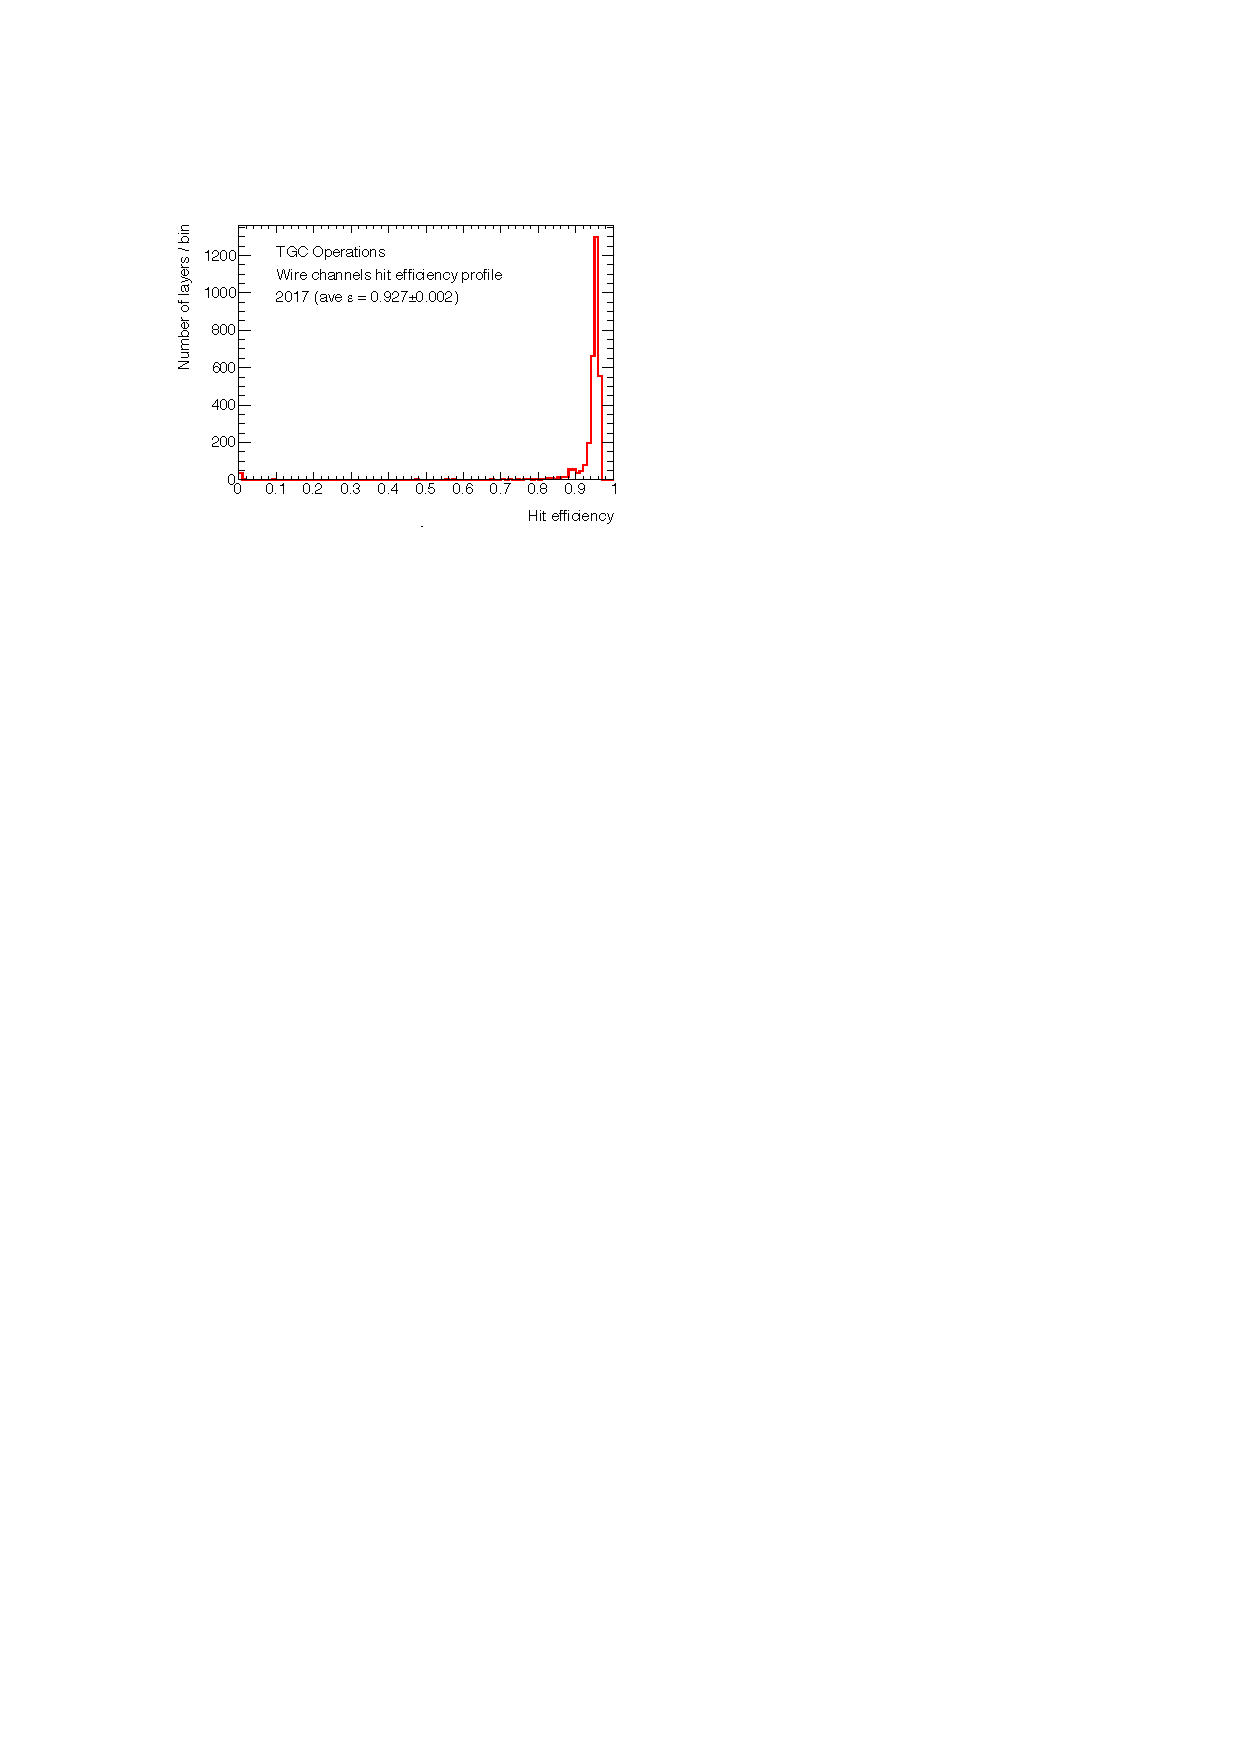
\includegraphics[height=5cm]{fig/Test/tgchit_wire.pdf}
\subcaption{ワイヤー}
\end{minipage}%
\begin{minipage}[b]{.5\linewidth}
\centering
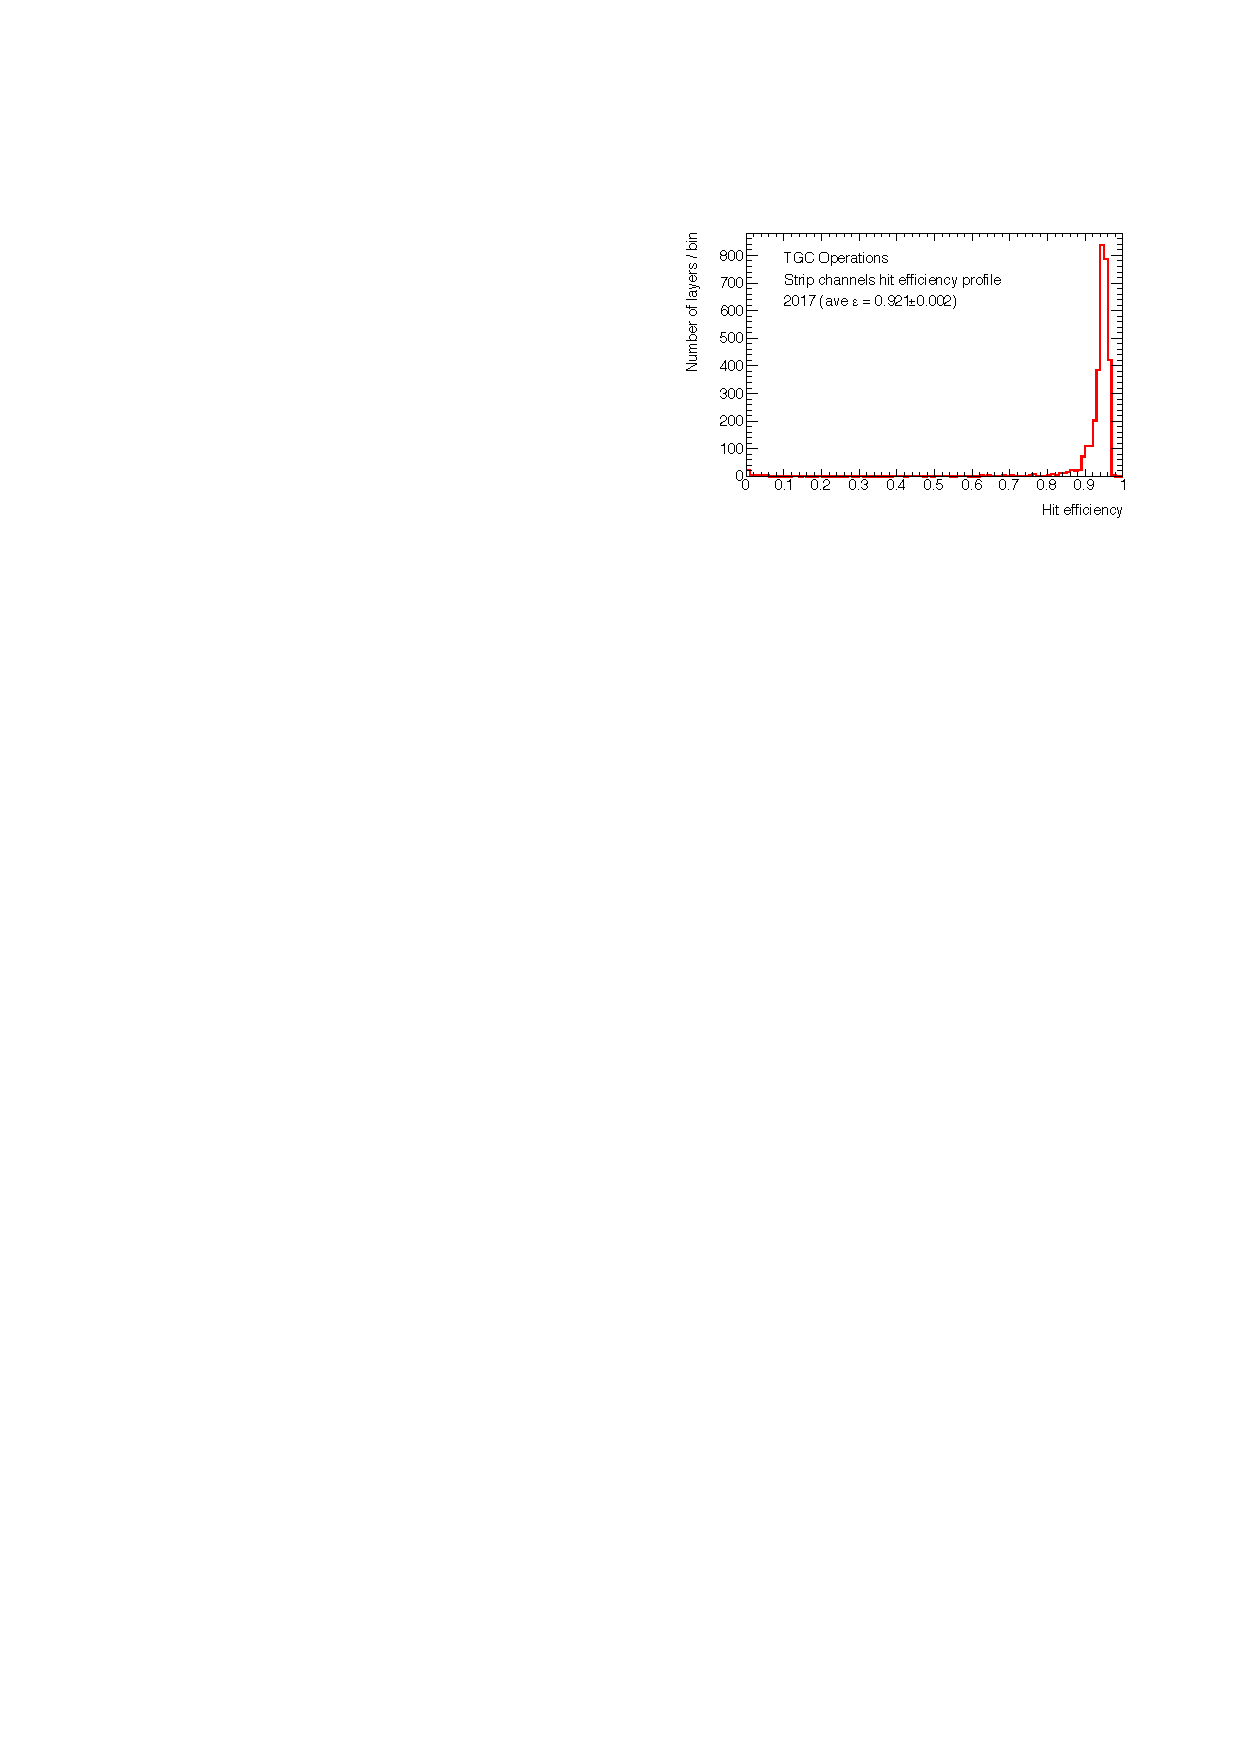
\includegraphics[height=5cm]{fig/Test/tgchit_strip.pdf}
\subcaption{ストリップ}
\end{minipage}%
\caption[2017年運転における TGC 各層のヒット検出効率]{2017年運転における TGC 各層のヒット検出効率\cite{mt_kawaguchi}。一枚のガスレイヤーにおける検出効率の平均はワイヤーで92.7 \%、ストリップで92.1 \%である。}
\label{tgchit_efficiency}
\end{figure}

2つ目は、多重散乱や制動放射に起因するInefficiencyである。多重散乱によりミューオン飛跡が途中で大角度に屈折したり、制動放射で生じた光子から電磁シャワーが生じ大量のヒットがTGCに残される場合には、Segment Reconstructionで正しい飛跡を再構成できなくなる。このようなイベントの例を図\ref{Brems}に示す。この図は実際のシングルミューオンモンテカルロサンプルに含まれる、TGCのヒット情報を3次元的にプロットしたものである。$x$軸と$y$軸にヒットのあった座標位置、$z$方向にTGCのレイヤー番号を示す。$z$座標が小さい方から大きい方にミューオンが入射し、ヒットを残した3次元座標をプロットしている。赤色の点がWireのヒットで青色がStripのヒット情報を表す。この図から、このイベントでは3層目でミューオンが制動放射を起こし、それに起因する電磁シャワーが4層目以降に複数のヒットを残していると考えられる。

\begin{figure} 
\centering
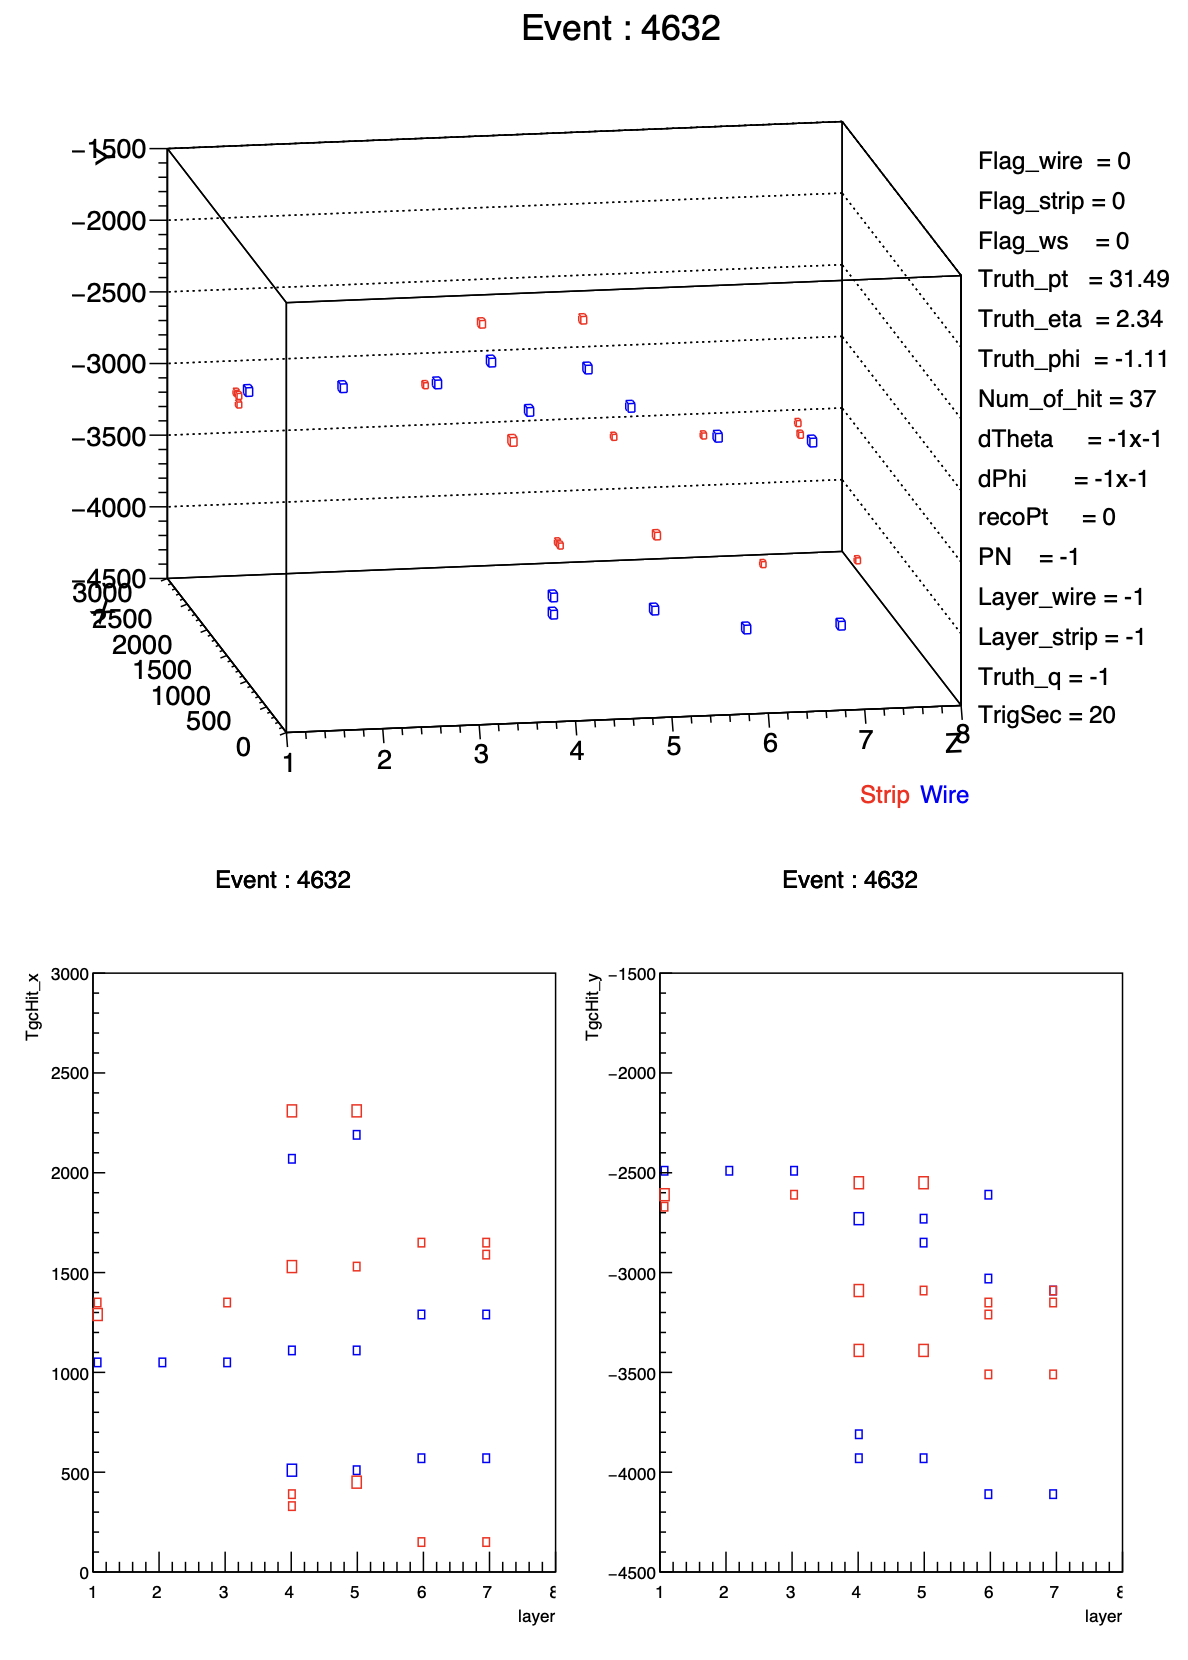
\includegraphics[width=16cm]{fig/Test/Brems.png}
\caption[制動放射が生じたと思われるイベントディスプレイ]{制動放射が生じたと思われるイベントディスプレイ。$x$軸と$y$軸にヒットのあった座標位置、$z$方向にTGCのレイヤー番号を示す。$z$座標が小さい方から大きい方にミューオンが入射し、ヒットを残した3次元座標をプロットしている。赤色の点がWireのヒットで青色がStripのヒット情報を表す。この図から、このイベントでは3層目でミューオンが制動放射を起こし、それに起因する電磁シャワーが4層目以降に複数のヒットを残していると考えられる。}
\label{Brems}
\end{figure}

Wire Strip Coincidenceで見られた6 \%のInefficiencyがどのような理由で生じているか調査するため、実機試験で飛跡再構成に失敗したイベントに対してイベントディスプレイを作成し、アイスキャンで原因の分類を行った。

データセットとして、フォワード領域のシングルミューオンイベントを10,000イベント用意した。このうちWire Strip Coincidenceで飛跡再構成に失敗したイベントは合計 583 イベントだった。
アイスキャンの結果を表\ref{tab:eyscan}に示す。プラトー領域における6 \%程度のInefficiencyのうち、ヒットレイヤーが少ないいことによるものが3割、多重散乱や制動放射によルものが3割、原理的な困難はなくLUTの調整などにより解決できる可能性があるものが4割程度であるとわかった。

\begin{table}[]
  \centering
  \caption{Wire Strip Coincidenceで飛跡再構成に失敗したイベントの調査結果}
  \label{tab:eyscan}
  \begin{tabular}{|c|c|}
  \hline
  飛跡再構成の原因                        & イベント数       \\ \hline\hline
  ヒットを残したレイヤーが少なく原理的に飛跡再構成ができないもの & 169 / 10000 \\ \hline
  多重散乱や制動放射により正しく飛跡を再構成することが困難なもの & 181 / 10000 \\ \hline
  その他 (アイスキャンでは原因を判断できなかったものを含む)  & 233 / 10000 \\ \hline
  合計                              & 583 / 10000 \\ \hline
  \end{tabular}
\end{table}


% \section{アライメントのずれに対するInefficiencyの考察}
% \label{sec:appendix:alignment}
% モンテカルデータはTGC検出器が、設計通りの理想位置に設置されていることを仮定して作成されたデータセットである。しかし、実際のTGC検出器はアライメントのずれにより、理想位置からずれた位置に設置されている。年度末のメンテナンス期間にはTGC検出器は一時移動し、再設置されるため、その度ごとにアライメントのずれが生じる。TGCトリガーロジックではチャンネルのヒット位置をもとに角度情報を算出するため、このアライメントのずれは角度再構成や\pt 再構成に影響を与える。特にその影響が顕著なWire Segment Reconstructionではこのずれを吸収するために、アライメントが行われるごとに新しくLUTを作成する予定である。しかし、これまでにアライメントのずれがどれだけトリガー性能に影響を与えるか評価されたことがない。
% そこで本研究では、シングルモンテカルロデータを用いて、アライメントのずれを考慮した場合と、考慮しない場合でどれだけ検出効率に差が生じるか測定した。
% 具体的には理想位置のジオメトリをもとに作成されたシングルミューオンイベントに対し、理想位置のジオミトリをもとに作成したLUTを使用してWire Segment Reconstructionを走らせた場合とと、2022年のアライメント後のジオミトリ情報をもとに作成したLUTを使用した場合とを比較する。

% 図\ref{alignment_wire}にWire Segment Reconstruction検出効率を示す。
% アライメントのずれを考慮した場合と考慮しない場合で、数\%程度検出効率に差が生じることがわかった。特に、フォワード領域ではジオミトリのずれによるInefficiencyが顕著な様子が窺える。

% \begin{figure} 
% \centering
% 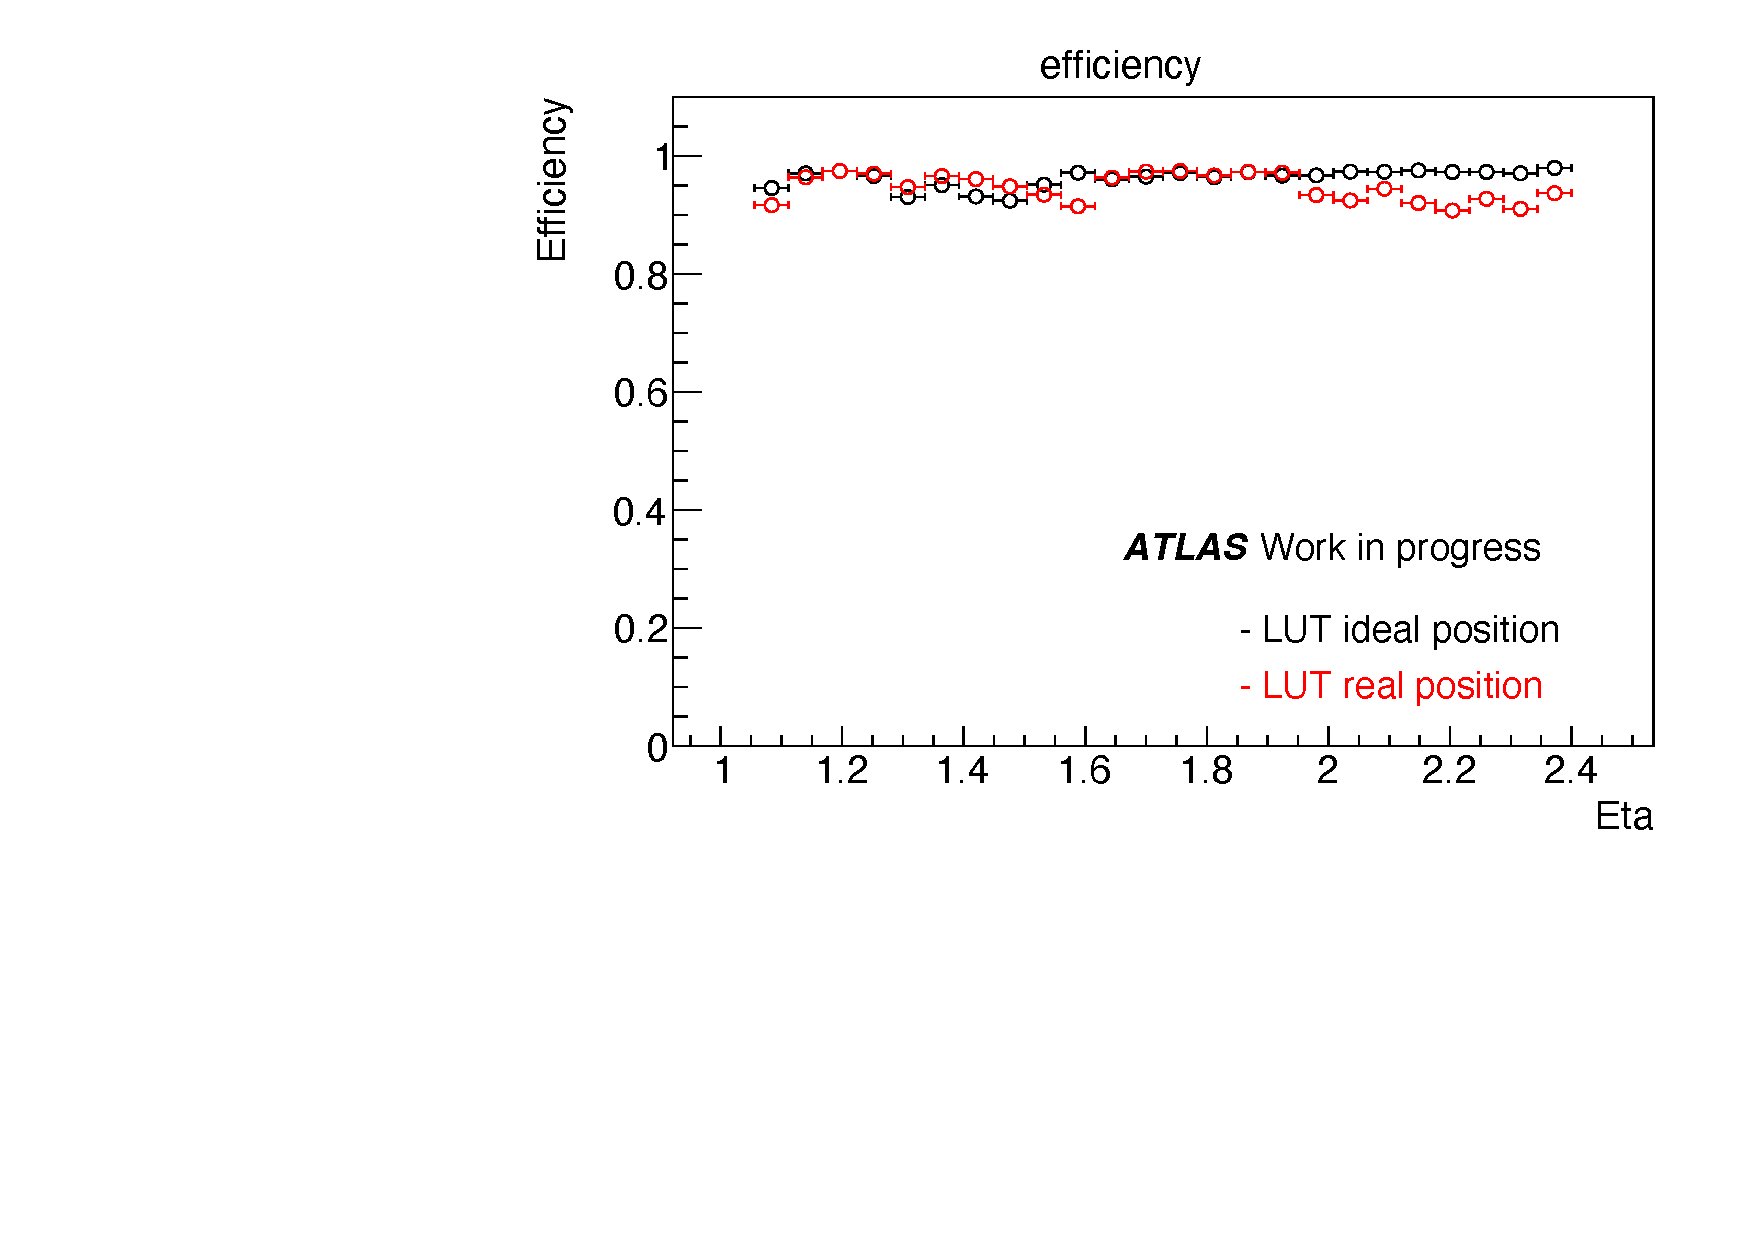
\includegraphics[width=16cm]{fig/Test/alignment_wire.pdf}
% \caption[]{理想位置のジオミトリを仮定したLUTと、2022年の実際のアライメントを考慮した場合のWire Segment Reconstructionの飛跡再構成効率の比較}
% \label{alignment_wire}
% \end{figure}

% 図\ref{alignment_ws}にWire Strip Coincidenceの\pt 閾値20 GeVに対するトリガー効率を示す。アライメントを考慮したLUTではTruth Muon \pt が20 GeVより小さいイベントに対して、不当に高い検出効率を持ってしまっていることがわかる。これはアライメントのずれによる角度再構成の不正確さが、角度を本来よりも小さく見積もる方向に働いた結果であると推測される。このように\pt 分解能が落ちると、物理的に興味のある\pt が高いイベントのみを選択するというトリガー本来の役割を果たせない。
% この結果では、アライメントを考慮したLUTを作成することが必要であると結論付けられる。

% \begin{figure} 
% \centering
% 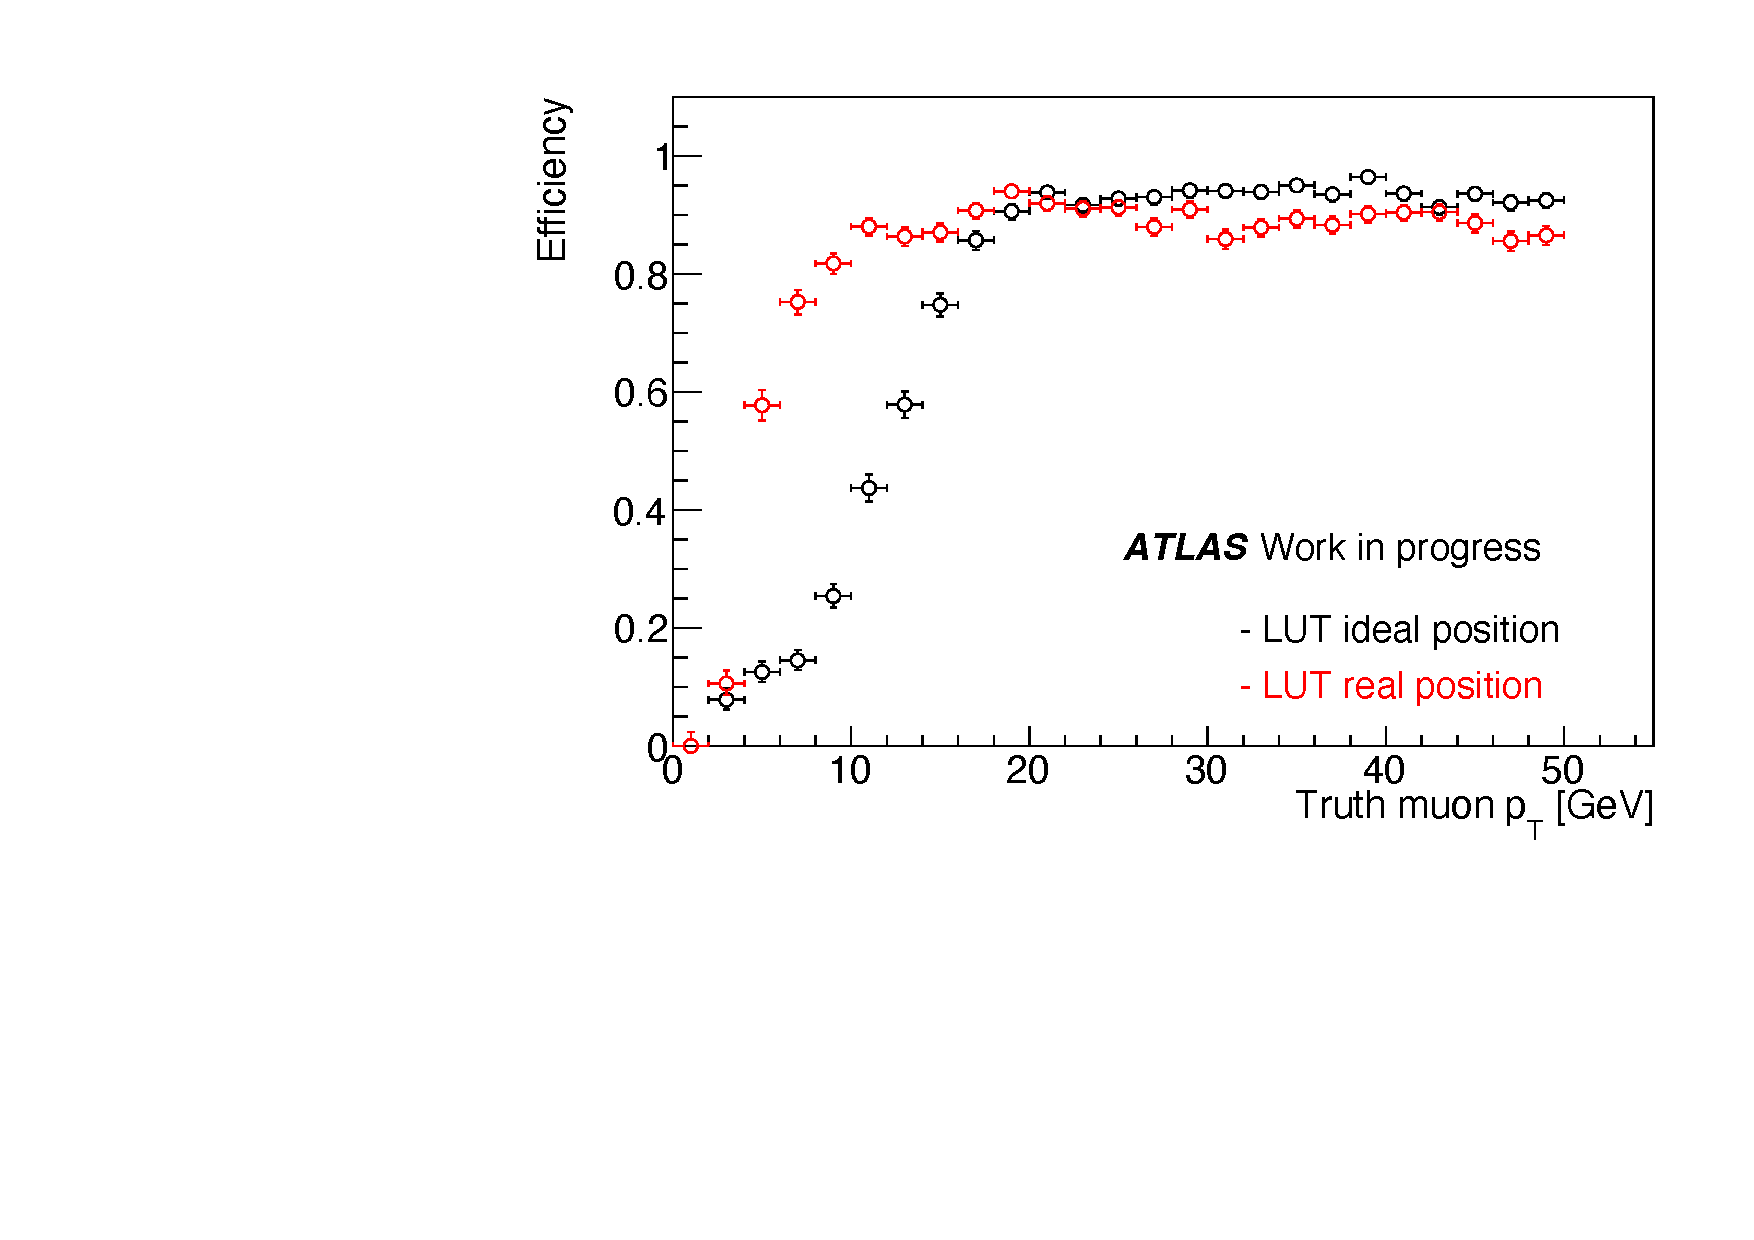
\includegraphics[width=16cm]{fig/Test/alignment_ws.pdf}
% \caption[CTAの完成想像図]{理想位置のジオミトリを仮定したLUTと、2022年の実際のアライメントを考慮した場合のWire Strip Coincidenceの飛跡再構成効率の比較}
% \label{alignment_ws}
% \end{figure}


